% !TEX root = saveliev_physics_general_course_1.tex
%!TEX TS-program = pdflatex
%!TEX encoding = UTF-8 Unicode


\chapter{MECHANICS OF A RIGID BODY}\label{chap:5}

\section{Motion of a Body}\label{sec:5_1}

In Sec.~\ref{sec:1_1}, we acquainted ourselves with the two fundamental kinds of motion of a rigid body---translation and rotation.

In translation, all the points of a body receive displacements equal in magnitude and direction during the same time interval. Consequently, the velocities and accelerations of all the points are identical at every moment of time. It is therefore sufficient to determine the motion of one of the points of a body (for example, of its centre of mass) to completely characterize the motion of the entire body.

In rotation, all the points of a rigid body move along circles whose centres are on a single straight line called the axis of rotation. To describe rotation, we must set the position of the axis of rotation in space and the angular velocity of the body at each moment of time.

Any motion of a rigid body can be represented as the superposition of the two fundamental kinds of motion indicated above. We shall show this for plane motion, \ie, motion when all the points of a body move in parallel planes. An example of plane motion is the rolling of a cylinder along a plane (\fig{5_1}).

\begin{figure}[t]
	\begin{minipage}[t]{0.5\linewidth}
		\begin{center}
			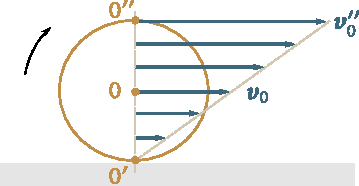
\includegraphics[scale=0.95]{figures/ch_05/fig_5_1.pdf}
			\caption[]{}
			\label{fig:5_1}
		\end{center}
	\end{minipage}
	\hspace{-0.05cm}
	\begin{minipage}[t]{0.5\linewidth}
		\begin{center}
			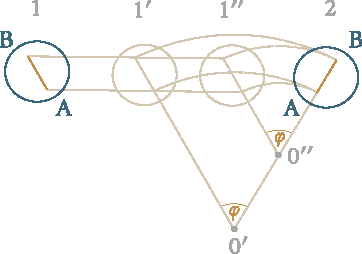
\includegraphics[scale=0.95]{figures/ch_05/fig_5_2.pdf}
			\caption[]{}
			\label{fig:5_2}
		\end{center}
	\end{minipage}
\vspace{-0.7cm}
\end{figure}

The arbitrary displacement of a rigid body from position $1$ to position $2$ (\fig{5_2}) can be represented as the sum of two displacements---translation from position $1$ to position $1'$ or $1''$, and rotation about the axis $0'$ or the axis $0''$. It is quite obvious that such a division of a displacement into translation and rotation can be performed in an infinite multitude of ways, but in any case rotation occurs through the same angle $\varphi$.

In accordance with the above, the elementary displacement of a point of a body ds can be resolved into two displacements---the ``translational'' one $\deriv{\vec{s}}_{\text{tr}}$ and the ``rotational'' one $\deriv{\vec{s}}_{\text{rot}}$:
\begin{equation*}
\deriv{\vec{s}} = \deriv{\vec{s}}_{\text{tr}} + \deriv{\vec{s}}_{\text{rot}}
\end{equation*}

\noindent
where $\deriv{\vec{s}}_{\text{tr}}$ is the same for all the points of the body. This resolution of the displacement $\deriv{\vec{s}}$, as we have seen, can be performed in different ways. In each of them, the rotational displacement $\deriv{\vec{s}}_{\text{rot}}$ is performed by rotation of the body through the same angle $\deriv{\varphi}$ (but relative to different axes), whereas $\deriv{\vec{s}}_{\text{tr}}$ and $\deriv{\vec{s}}_{\text{rot}}$ are different.

Dividing $\deriv{\vec{s}}$ by the corresponding time interval $\deriv{t}$, we get the velocity of a point:
\begin{equation*}
\vec{v} = \diff{\vec{s}}{t} = \frac{\deriv{\vec{s}_{\text{tr}}}}{t} + \frac{\deriv{\vec{s}_{\text{rot}}}}{t} = \vec{v}_0 + \vec{v}'
\end{equation*}

\noindent
where $\vec{v}_0$ is the velocity of translation, which is the same for all the points of a body, $\vec{v}'$ is the velocity due to rotation, which is different for different points of the body.

Thus, the plane motion of a rigid body can be represented as the sum of two motions---translation with the velocity $\vec{v}_0$ and rotation with the angular velocity $\vec{\omega}$ (the vector $\vec{\omega}$ in \fig{5_1} is directed at right angles to the plane of the drawing, beyond it). Such a representation of complex motion can be accomplished in many ways differing in the values of $\vec{v}_0$ and $\vec{v}'$, but corresponding to the same angular velocity $\vec{\omega}$. For example, the motion of a cylinder rolling without slipping along a plane (\fig{5_1}) can be represented either as translation with the velocity $\vec{v}_0$ and simultaneous rotation with the angular velocity $\vec{\omega}$ about the axis $0$, or as translation with the velocity $\vec{v}_0''=2\vec{v}_0$ and rotation with the same angular velocity $\vec{\omega}$ about the axis $0''$, or, finally, as only rotation, again with the same angular velocity $\vec{\omega}$ about the axis $0'$.

Assuming that the reference frame relative to which we are considering the complex motion of a rigid body is stationary, the motion of the body can be represented as rotation with the angular velocity $\vec{\omega}$ in a reference frame moving translationally with the velocity $\vec{v}_0$ relative to the stationary frame.

The linear velocity $\vec{v}'$ of a point with the position vector $\vec{r}$ due to rotation of a rigid body is $\vec{v}'=\vecprod{\omega}{r}$ [see~\eqn{1_100}]. Consequently, the velocity of this point in complex motion can be represented in the form
\begin{equation}\label{eq:5_1}
\vec{v} = \vec{v}_0 + \vecprod{\omega}{r}.
\end{equation}

An elementary displacement of a rigid body in plane motion can always be represented as rotation about an axis called the \textbf{instantaneous axis of rotation}. This axis may be either inside the body or outside it. The position of the instantaneous axis of rotation relative to a fixed reference frame and relative to the body itself, generally speaking, changes with time. For a rolling cylinder (\fig{5_2}), the instantaneous axis $0'$ coincides with the line of contact of the cylinder with the plane. When the cylinder rolls, the instantaneous axis moves both along the plane (\ie, relative to a fixed reference frame) and along the surface of the cylinder.

The velocities of all the points of the body for each moment of time can be considered as due to rotation about the corresponding instantaneous axis. Consequently, plane motion of a rigid body can be considered as a number of consecutive elementary rotations about instantaneous axes.

In non-planar motion, an elementary displacement of a body can be represented as rotation about an instantaneous axis only if the vectors $\vec{v}_0$ and $\vec{\omega}$ are mutually perpendicular. If the angle between these vectors differs from $\pi/2$, the motion of the body at each moment of time will be the superposition of two motions---rotation about a certain axis, and translation along this axis.

\section{Motion of the Centre of Mass of a Body}\label{sec:5_2}

By dividing a body into elementary masses $m_i$ we can represent it as a system of point particles whose mutual arrangement remains unchanged. Any of these elementary masses may be acted upon both by internal forces due to its interaction with other elementary masses of the body being considered, and by external forces. For example, if a body is in the field of the Earth's gravitational forces, each elementary mass of the body $m_i$ will experience an external force equal to $m\vec{g}$.

Let us write the equation of Newton's second law for each elementary mass:
\begin{equation}\label{eq:5_2}
m_i\vec{a}_i = \vec{f}_i + \vec{F}_i
\end{equation}

\noindent
where $\vec{f}_i$ is the resultant of all the internal forces, and $\vec{F}_i$ the resultant of all the external forces applied to the given elementary mass. Summation of Eqs.~\eqref{eq:5_2} for all the elementary masses yields
\begin{equation}\label{eq:5_3}
	\sum_i m_i\vec{a}_i = \sum_i \vec{f}_i + \sum_i \vec{F}_i.
\end{equation}

\noindent
The sum of all the internal forces acting in a system, however, equals zero. Hence, \eqn{5_3} can be simplified as follows:
\begin{equation}\label{eq:5_4}
	\sum_i m_i\vec{a}_i = \sum_i \vec{F}_i.
\end{equation}

\noindent
Here the resultant of all the external forces acting on the body is in the right-hand side.

The sum in the left-hand side of \eqn{5_4} can be replaced with the product of the mass of the body $m$ and the acceleration of its centre of mass (centre of inertia) $\vec{a}_{\text{C}}$. Indeed, according to \eqn{3_91}, we have
\begin{equation*}
	\sum_i m_i\vec{r}_i = m \vec{r}_{\text{C}}.
\end{equation*}

\noindent
Differentiating this relation twice with respect to time and taking into account that $\ddot{\vec{r}}_i=\vec{a}_i$, and $\ddot{\vec{r}}_{\text{C}}=\vec{a}_{\text{C}}$, we can write
\begin{equation}\label{eq:5_5}
	\sum_i m_i\vec{a}_i = m \vec{a}_{\text{C}}.
\end{equation}

Comparing Eqs.~\eqref{eq:5_4} and \eqref{eq:5_5}, we arrive at the equation
\begin{equation}\label{eq:5_6}
	m \vec{a}_{\text{C}} = \sum\vec{F}_{\text{ext}}
\end{equation}

\noindent
which signifies that \textit{the centre of mass of a rigid body moves in the same way as a point particle of a mass equal to that of the body would move under the action of all the forces applied to the body}.

Equation~\eqref{eq:5_6} permits us to find the motion of the centre of mass of a rigid body if we know the mass of the body and the forces acting on it. For translation, this equation will determine the acceleration not only of the centre of mass, but also of any other point of the body.

\section{Rotation of a Body about a Fixed Axis}\label{sec:5_3}

Let us consider a rigid body that can rotate about a fixed vertical axis (\fig{5_3}). We shall confine the axis in bearings to prevent its displacements in space. The flange $Fl$ resting on the lower bearing prevents motion of the axis in a vertical direction.

\begin{figure}[t]
	\begin{minipage}[t]{0.5\linewidth}
		\begin{center}
			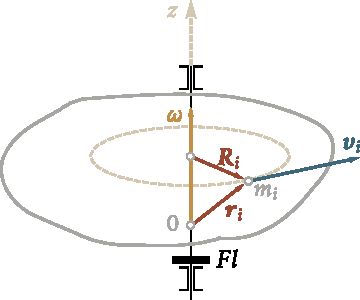
\includegraphics[scale=0.95]{figures/ch_05/fig_5_3.pdf}
			\caption[]{}
			\label{fig:5_3}
		\end{center}
	\end{minipage}
	\hspace{-0.05cm}
	\begin{minipage}[t]{0.5\linewidth}
		\begin{center}
			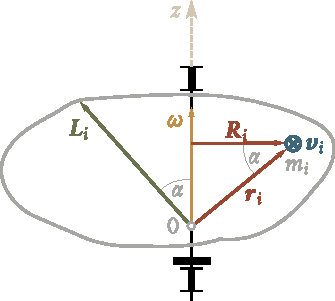
\includegraphics[scale=0.95]{figures/ch_05/fig_5_4.pdf}
			\caption[]{}
			\label{fig:5_4}
		\end{center}
	\end{minipage}
\vspace{-0.5cm}
\end{figure}

A perfectly rigid body can be considered as a system of particles (point particles) with constant distances between them. Equation~\eqref{eq:3_118}, \ie,
\begin{equation*}
\diff{\vec{L}}{t} = \sum \vec{M}_{\text{ext}}
\end{equation*}

\noindent
holds for any system of particles, including a rigid body. In the latter case, $\vec{L}$ is the angular momentum of the body. The right-hand side of \eqn{3_118} is the sum of the moments of the external forces acting on the body.

Let us take point $0$ on the axis of rotation and characterize the position of the particles forming the body with the aid of position vectors $\vec{r}$ drawn from this point (\fig{5_3} depicts the $i$-th particle of mass $m_1$). According to \eqn{3_105}, the angular momentum of the $i$-th particle relative to point $0$ is
\begin{equation}\label{eq:5_7}
\vec{L}_i = \vec{r}_i \times m_i\vec{v}_i = m_i\vecprodind{r}{i}{v}{i}.
\end{equation}

\noindent
The vectors $\vec{r}_i$ and $\vec{v}_i$ are mutually perpendicular for all the particles of the body. Therefore, the magnitude of the vector $\vec{L}_i$ [\eqn{5_7}] is
\begin{equation}\label{eq:5_8}
L_i = m_i r_i v_i = m_i r_i \omega R_i
\end{equation}

\noindent
[see \eqn{1_99}]. The direction of the vector $\vec{L}_i$ is shown in \fig{5_4}. It must be noted that the ``length'' of the vector $\vec{L}_i$, according to \eqn{5_8}, is proportional to the velocity of rotation of the body $\vec{\omega}$. The direction of the vector $\vec{L}_i$, however, is independent of $\vec{\omega}$. The vector $\vec{L}_i$ is in a plane passing through the axis of rotation and the particle $m_i$ and is perpendicular to $\vec{r}_i$.

The projection of the vector $\vec{L}_i$ onto the axis of rotation (the $z$-axis), as can be seen from \fig{5_4}, is [see \eqn{5_8}]
\begin{equation}\label{eq:5_9}
L_{zi} = L_i\cos\alpha = m_i r_i \omega R_i \cos\alpha = m_i(r_i\cos\alpha)R_i\omega = m_iR_i^2\omega.
\end{equation}

\begin{figure}[t]
	\begin{center}
		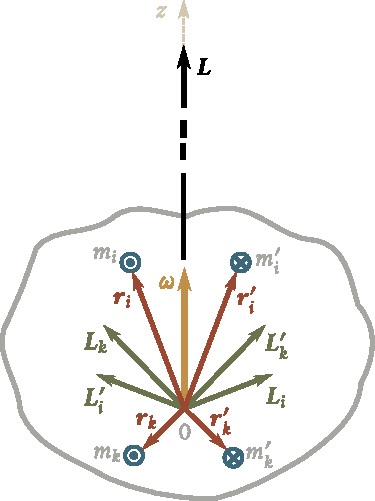
\includegraphics[scale=0.95]{figures/ch_05/fig_5_5.pdf}
		\caption[]{}
		\label{fig:5_5}
	\end{center}
\vspace{-1.0cm}
\end{figure}

It is not difficult to see that for a homogeneous\footnote{In mechanics, a body is defined as homogeneous when its density is the same throughout the entire volume (see Sec.~\ref{sec:5_4}).} body which is symmetrical relative to the axis of rotation (for a homogeneous body of revolution), the directions of the total angular momentum (equal to $\sum_i\vec{L}_i$) and of $\vec{\omega}$ along the axis of rotation are the same (\fig{5_5}). Indeed, in this case, the body can be divided into pairs of symmetrically arranged particles of equal mass (two pairs of particles are shown in the figure---$m_i$-$m_i'$ and $m_k$-$m_k'$). The sum of the angular momenta of each pair (in the figure $\vec{L}_i+\vec{L}_i'$ and $\vec{L}_k+\vec{L}_k'$) is directed along the vector $\vec{\omega}$. Hence, the total angular momentum $\vec{L}$ will also coincide in direction with $\vec{\omega}$. The magnitude of the vector $\vec{L}$ in this case equals the sum of the projections of the momenta $\vec{L}_i$ onto the $z$-axis. Taking \eqn{5_9} into account, we get the following expression for the magnitude of the angular momentum of a body:
\begin{equation}\label{eq:5_10}
L = \sum_i L_{zi} = \omega \sum_i m_i R_i^2 = I \omega.
\end{equation}

\noindent
The quantity $I$ equal to the sum of the products of the elementary masses and the squares of their distances from a certain axis is called the \textbf{rotational inertia} or the \textbf{moment of inertia of the body} relative to the given axis:
\begin{equation}\label{eq:5_11}
I = \sum_i m_i R_i^2.
\end{equation}

\noindent
Summation is performed over all the elementary masses $m_i$ into which the body was mentally divided.

\begin{figure}[t]
	\begin{minipage}[t]{0.5\linewidth}
		\begin{center}
			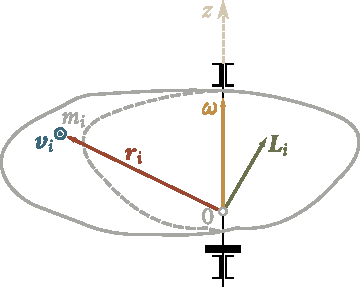
\includegraphics[scale=0.95]{figures/ch_05/fig_5_6.pdf}
			\caption[]{}
			\label{fig:5_6}
		\end{center}
	\end{minipage}
	\hspace{-0.05cm}
	\begin{minipage}[t]{0.5\linewidth}
		\begin{center}
			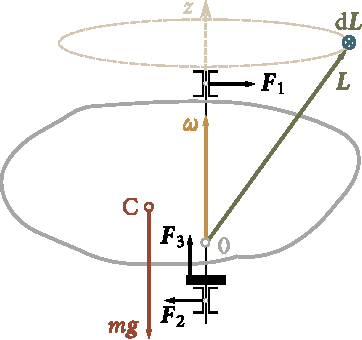
\includegraphics[scale=0.95]{figures/ch_05/fig_5_7.pdf}
			\caption[]{}
			\label{fig:5_7}
		\end{center}
	\end{minipage}
\vspace{-0.7cm}
\end{figure}

With a view to the fact that the vectors $\vec{L}$ and $\vec{\omega}$ have identical directions, we can write \eqn{5_10} as follows:
\begin{equation}\label{eq:5_12}
\vec{L} = I \vec{\omega}.
\end{equation}

\noindent
We remind our reader that we have obtained this relation for a homogeneous body rotating about an axis of symmetry. In the general case, as we shall see below, \eqn{5_12} is not obeyed.

For an asymmetrical (or non-homogeneous) body, the angular momentum $\vec{L}$, generally speaking, does not coincide in direction with the vector $\vec{\omega}$. The dash line in \fig{5_6} shows the part of an asymmetrical homogeneous body that is symmetrical relative to the axis of rotation. The total angular momentum of this part, as we have established above, is directed along $\vec{\omega}$. The momentum $\vec{L}_i$ of each particle not belonging to the symmetrical part deviates to the right from the axis of rotation (in a plane figure). Consequently, the total angular momentum of the entire body will also deviate to the right (\fig{5_7}). Upon rotation of the body, the vector $\vec{L}$ rotates together with it, describing a cone. During the time $\deriv{t}$, the vector $\vec{L}$ receives the increment $\deriv{\vec{L}}$, which according to \eqn{3_118} equals
\begin{equation}\label{eq:5_13}
\deriv{\vec{L}} = \left( \sum \vec{M}_{\text{ext}} \right) \, \deriv{t}.
\end{equation}

\noindent
If the vector $\vec{L}$ does not change in magnitude, then the vector $\deriv{\vec{L}}$ is directed beyond the drawing (\fig{5_7}). The vector $\sum\vec{M}_{\text{ext}}$ has the same direction. In the example we are treating, the moments of the external forces include (1) the moment of the force of gravity $m\vec{g}$ directed toward us---we shall call it negative (this force is applied to the centre of mass of the body C), (2) the positive moments of the forces of lateral pressure of the bearings on the axis (the forces $\vec{F}_1$ and $\vec{F}_2$), and (3) the positive moment of the force of pressure of the bearing shoulder on the flange $\vec{F}_3$. We assume that friction forces are absent, otherwise the vector $\vec{L}$ would not be constant in magnitude, and $\deriv{\vec{L}}$ would not be perpendicular to $\vec{L}$.

The angular momentum relative to the axis of rotation [see \eqn{3_108}] for any (homogeneous or non-homogeneous, symmetrical or asymmetrical) body is
\begin{equation}\label{eq:5_14}
L_z = \sum_i L_{zi} = \sum_i m_i R_i^2 \omega = I \omega
\end{equation}

\noindent
(see Eqs.~\eqref{eq:5_9} and \eqref{eq:5_11}]. It must be stressed that unlike \eqn{5_12}, \eqn{5_14} is always correct.

Equation~\eqref{eq:3_119} states that
\begin{equation*}
\diff{L_z}{t} = \sum M_{z,\text{ext}}.
\end{equation*}

\noindent
Introducing into this expression \eqn{5_14} for $L_z$, we get
\begin{equation}\label{eq:5_15}
I \alpha_z = \sum M_{z,\text{ext}}
\end{equation}

\noindent
where $\alpha_z=\dot{\omega}$ is the projection of the angular acceleration onto the $z$-axis (we are considering rotation about a fixed axis, therefore the vector $\vec{\omega}$ can change only in magnitude). Equation~\eqref{eq:5_15} is similar to the equation $m\vec{a}=\vec{F}$. The part of the mass is played by the moment of inertia, that of the linear acceleration by the angular acceleration, and, finally, the part of the resultant force is played by the total moment of the external forces.

In the above example, the moments of all the external forces are perpendicular to the axis of rotation. Hence, their projections onto the $z$-axis equal zero. Accordingly, the angular velocity $\vec{\omega}$ remains constant, which is what should be expected in the absence of friction.

We must point out that in the rotation of a homogeneous symmetrical body, forces of lateral pressure of the bearings on the axis (the forces $\vec{F}_1$ and $\vec{F}_2$ in \fig{5_7}) do not appear. In the absence of the force of gravity, we could remove the bearings---the axis would retain its position in space without them. An axis whose position in space remains constant when bodies rotate about it in the absence of external forces is called a \textbf{free axis} of a body.

It is possible to prove that for a body of any shape and with an arbitrary arrangement of its mass there are three mutually perpendicular axes passing through the centre of mass of the body that can be free axes. They are called the \textbf{principal axes} of inertia of the body.

\begin{figure}[t]
	\begin{minipage}[t]{0.5\linewidth}
		\begin{center}
			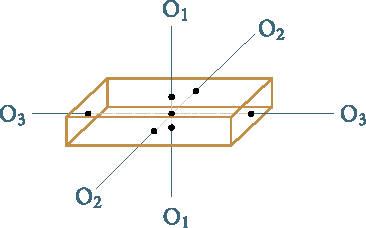
\includegraphics[scale=0.98]{figures/ch_05/fig_5_8.pdf}
			\caption[]{}
			\label{fig:5_8}
		\end{center}
	\end{minipage}
	\hspace{-0.05cm}
	\begin{minipage}[t]{0.5\linewidth}
		\begin{center}
			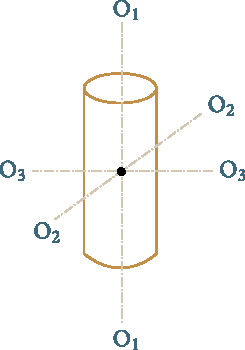
\includegraphics[scale=0.95]{figures/ch_05/fig_5_9.pdf}
			\caption[]{}
			\label{fig:5_9}
		\end{center}
	\end{minipage}
\vspace{-0.7cm}
\end{figure}

In a homogeneous parallelepiped (\fig{5_8}), the principal axes of inertia are obviously the axes O$_1$O$_1$, O$_2$O$_2$, and O$_3$O$_3$ passing through the centres of opposite faces.

In bodies possessing axial symmetry (for example, in a homogeneous\footnote{It is sufficient that the density of the body in each cross section be a function only of the distance from the axis of symmetry.} cylinder), the axis of symmetry is one of the principal axes of inertia. Any two mutually perpendicular axes in a plane at right angles to the axis of symmetry and passing through the centre of mass of the body can be the other two principal axes (\fig{5_9}). Thus, in such a body only one of the principal axes of inertia is fixed.

In a body with central symmetry, \ie, in a sphere whose density depends only on the distance from its centre, any three mutually perpendicular axes passing through the centre of mass are the principal axes of inertia. Consequently, none of the principal axes of inertia is fixed.

The moments of inertia relative to the principal axes are called the \textbf{principal moments of inertia} of a body. In the general case, these moments differ: $I_1\neq I_2\neq I_3$. For a body with axial symmetry, two of the principal moments of inertia are the same, while the third one, generally speaking, differs from them: $I_1=I_2\neq I_3$. And, finally, for a body with central symmetry, all three principal moments of inertia are the same: $I_1=I_2=I_3$.

Not only a homogeneous sphere, but also, for instance, a homogeneous cube has equal values of the principal moments of inertia. In the general case, such equality may be observed for bodies of an absolutely arbitrary shape when their mass is properly distributed. All such bodies are called \textbf{spherical tops}. Their feature is that any axis passing through their centre of mass has the properties of a free axis, and, consequently, none of the principal axes is fixed, as for a sphere. All spherical tops behave the same when they rotate in identical conditions.

Bodies for which $I_1=I_2\neq I_3$ behave like homogeneous bodies of revolution. They are called \textbf{symmetrical tops}. Finally, bodies for which $I_1=I_2=I_3$ are called \textbf{asymmetrical tops}.

If a body rotates in conditions when there is no external action, then only rotation about the principal axes corresponding to the maximum and minimum values of the moment of inertia is stable. Rotation about an axis corresponding to an intermediate value of the moment will be unstable. This signifies that the forces appearing upon the slightest deviation of the axis of rotation from this principal axis act in a direction causing the magnitude of this deviation to grow. When the axis of rotation deviates from a stable axis, the forces produced return the body to rotation about the corresponding principal axis.

\begin{figure}[t]
	\begin{center}
		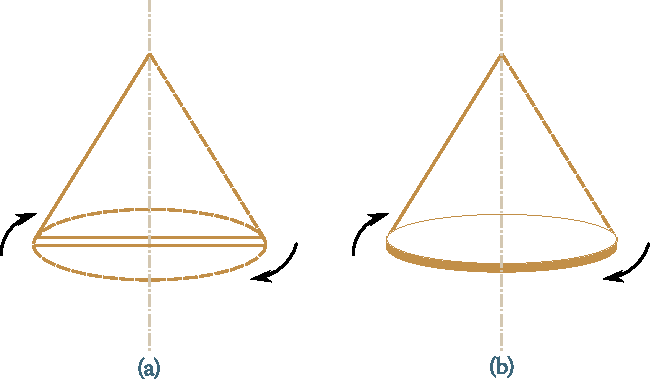
\includegraphics[scale=0.9]{figures/ch_05/fig_5_10.pdf}
		\caption[]{}
		\label{fig:5_10}
	\end{center}
\vspace{-1.0cm}
\end{figure}

We can convince ourselves that what has been said above is true by tossing a body having the shape of a parallelepiped (for example, a match box) and simultaneously bringing it into rotation\footnote{The action of the force of gravity in this case is not significant. It only causes the body to fall in addition to its rotation.}. We shall see that the body when falling can rotate stably about axes passing through the biggest or smallest faces. Attempts to toss the body so that it rotates about an axis passing through the faces of an intermediate size will be unsuccessful.

If an external force is exerted, for instance, by the string on which a rotating body is suspended, then only rotation about the principal axis corresponding to the maximum value of the moment of inertia will be stable. This is why a thin rod suspended by means of a string fastened to its end when brought into rapid rotation will in the long run rotate about an axis normal to it passing through its centre (\fig{5_10}a). A disk suspended by means of a string fastened to its edge (\fig{5_10}b) behaves in a similar way.

Up to now, we have treated bodies with a constant distribution of their mass. Now let us assume that a rigid body can lose for a certain time its property of a constant arrangement of its parts, and within this time redistribution of the body's mass occurs that results in the moment of inertia changing from $I_1$ to $I_2$. If such a redistribution occurs in conditions when $\sum\vec{M}_{\text{ext}}=0$, then in accordance with the law of conservation of angular momentum the following equation must be observed:
\begin{equation}\label{eq:5_16}
I_1\omega_1 = I_2\omega_2
\end{equation}

\noindent
where $\omega_1$ is the initial, and $\omega_2$ is the final value of the angular velocity of the body. Thus, a change in the moment of inertia leads to a corresponding change in the angular velocity. This explains why a spinning figure skater (or a man on a rotating platform) begins to rotate more slowly when he stretches his arms out, and gains speed when he presses his arms against his body.

\section{Moment of Inertia}\label{sec:5_4}

From the definition of the moment of inertia\footnote{In this section, it is expedient to use the symbol $\Delta m_i$ instead of $m_i$ for the elementary mass of a body.} [see \eqn{5_11}]
\begin{equation*}
I = \sum_i \Delta m_i R_i^2
\end{equation*}

\noindent
we can see that it is an additive quantity. This signifies that the moment of inertia of a body equals the sum of the moments of inertia of its parts.

We introduced the concept of the moment of inertia when dealing with the rotation of a rigid body. It must be borne in mind, however, that this quantity exists irrespective of rotation. Every body, regardless of whether it is rotating or at rest, has a definite moment of inertia relative to any axis, just like a body has a mass regardless of whether it is moving or at rest.

The distribution of the mass within a body can be characterized with the aid of a quantity called the density. If a body is homogeneous, \ie, its properties are the same at all of its points, then the density is defined as the quantity
\begin{equation}\label{eq:5_17}
\rho = \frac{m}{V}
\end{equation}

\noindent
where $m$ and $V$ are the mass and volume of the body, respectively. Thus, the density of a homogeneous body is the mass of a unit of its volume.

For a body with an unevenly distributed mass, \eqn{5_17} gives the average density. The density at a given point is determined in this case as follows:
\begin{equation}\label{eq:5_18}
\rho = \lim_{\Delta v\to 0} \frac{\Delta m}{\Delta V} = \diff{m}{V}.
\end{equation}

\noindent
In this expression, $\Delta m$ is the mass contained in the volume $\Delta V$, which in the limit transition contracts to the point at which the density is being determined.

The limit transition in \eqn{5_18} must not be understood in the sense that $\Delta V$ contracts literally to a point. If such a meaning is implied, we would get a greatly differing result for two virtually coinciding points, one of which is at the nucleus of an atom, while the other is at a space between nuclei (the density for the first point would be enormous, and for the second one it would be zero). Therefore, $\Delta V$ should be diminished until we get an infinitely small volume from the physical viewpoint. We understand this to mean such a volume which on the one hand is small enough for the macroscopic (\ie, belonging to a great complex of atoms) properties within its limits to be considered identical, and on the other hand is sufficiently great to prevent discreteness (discontinuity) of the substance from manifesting itself.

By \eqn{5_18}, the elementary mass $\Delta m_i$ equals the product of the density of a body $\rho_i$ at a given point and the corresponding elementary volume $\Delta V_i$:
\begin{equation*}
\Delta m_i = \rho_i \Delta V_i.
\end{equation*}

\noindent
Consequently, the moment of inertia can be written in the form
\begin{equation}\label{eq:5_19}
I = \sum_i \rho_i R_i^2 \Delta V_i.
\end{equation}

\noindent
If the density of a body is constant, it can be put outside the sum:
\begin{equation}\label{eq:5_20}
I = \rho \sum_i R_i^2 \Delta V_i.
\end{equation}

Equations~\eqref{eq:5_19} and \eqref{eq:5_20} are approximate. Their accuracy grows with diminishing elementary volumes $\Delta V_i$ and the elementary masses $\Delta m_i$ corresponding to them. Hence, the task of finding the moments of inertia consists in integration:
\begin{equation}\label{eq:5_21}
I = \int R^2\, \deriv{m} = \int \rho R^2\, \deriv{V}.
\end{equation}

\noindent
The integrals in \eqn{5_21} are taken over the entire volume of the body. The quantities $\rho$ and $R$ in these integrals are position functions, \ie, for example, functions of the Cartesian coordinates $x$, $y$, and $z$.

As an example, let us find the moment of inertia of a homogeneous disk relative to an axis perpendicular to the plane of the disk and passing through its centre (\fig{5_11}). Let us divide the disk into annular layers of thickness $\deriv{R}$. All the points of one layer will be at the same distance $R$ from the axis. The volume of such a layer is
\begin{equation*}
\deriv{V} = 2\pi bR\,\deriv{R}
\end{equation*}

\noindent
where $b$ is the thickness of the disk.

Since the disk is homogeneous, its density at all its points is the same, and $\rho$ in \eqn{5_21} can be put outside the integral:
\begin{equation*}
I = \rho \int R^2\,\deriv{V} = \rho \int_0^{R_0} R^2 2\pi bR\,\deriv{R}
\end{equation*}

\noindent
where $R_0$ is the radius of the disk. Let us put the constant factor $2\pi b$ outside the integral:
\begin{equation*}
I = 2\pi b\rho \int_0^{R_0} R^3\,\deriv{R} = 2\pi b\rho\frac{R^4_0}{4}.
\end{equation*}

\noindent
Finally, introducing the mass of the disk $m$ equal to the product of the density $\rho$ and the volume of the disk $b\pi R^2_0$, we get
\begin{equation}\label{eq:5_22}
I = \frac{mR_0^2}{2}.
\end{equation}

\begin{figure}[t]
	\begin{center}
		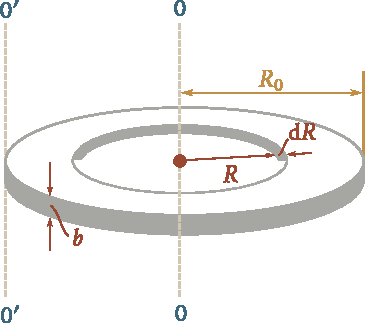
\includegraphics[scale=0.95]{figures/ch_05/fig_5_11.pdf}
		\caption[]{}
		\label{fig:5_11}
	\end{center}
\vspace{-1.0cm}
\end{figure}

The finding of the moment of inertia in the above example was simplified quite considerably owing to the fact that the body was homogeneous and symmetrical, and we sought the moment of inertia relative to an axis of symmetry. If we wanted to find the moment of inertia of the disk relative, for example, to the axis $0'0'$ perpendicular to the disk and passing through its edge (see \fig{5_11}), the calculations would evidently be much more complicated. The finding of the moment of inertia is considerably simplified in such cases if we use the Steiner or parallel axis theorem, which is formulated as follows: \textit{the moment of inertia $I$ relative to an arbitrary axis equals the moment of inertia $I_{\text{C}}$ relative to an axis parallel to the given one and passing through the body's centre of mass plus the product of the body's mass $m$ and the square of the distance $b$ between the axes}:
\begin{equation}\label{eq:5_23}
I = I_{\text{C}}= mb^2.
\end{equation}

According to the parallel axis theorem, the moment of inertia of the disk relative to the axis $0'0'$ equals the moment of inertia relative to the axis passing through the centre of the disk, which we have found [\eqn{5_22}] plus $mR_0^2$ (the distance between the axes $0'0'$ and $00$ equals the radius of the disk $R_0$):
\begin{equation*}
I = \frac{mR^2_0}{2} + mR_0^2 = \frac{3}{2}mR_0^2.
\end{equation*}

Thus, the parallel axis theorem in essence reduces the calculation of the moment of inertia relative to an arbitrary axis to the calculation of the moment of inertia relative to an axis passing through the centre of mass of the body.

\begin{figure}[t]
	\begin{center}
		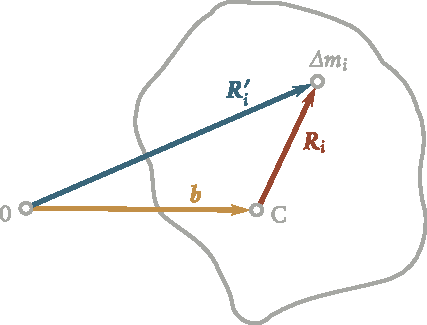
\includegraphics[scale=0.93]{figures/ch_05/fig_5_12.pdf}
		\caption[]{}
		\label{fig:5_12}
	\end{center}
\vspace{-1.0cm}
\end{figure}

To prove the parallel axis theorem, let us consider axis C passing through the centre of mass of a body and axis $0$ parallel to it and at a distance $b$ from axis C (\fig{5_12}, both axes are perpendicular to the plane of the drawing). Let $\vec{R}_i$ be a vector perpendicular to axis C and drawn from the axis to the elementary mass $\Delta m_i$ and $\Delta\vec{R}_i$ be a similar vector drawn from axis $0$. We shall also introduce the vector $\vec{b}$ perpendicular to the axes and connecting the corresponding points of axes $0$ and C. For any pair of points opposite each other, this vector has the same value (equal to the distance $b$ between the axes) and the same direction. The following relation holds between the vectors listed above:
\begin{equation*}
\vec{R}_i' = \vec{b} + \vec{R}_i.
\end{equation*}

The square of the distance to the elementary mass $\Delta m_i$ from axis C is $R_i^2=\vec{R}^2$, and from axis $0$ is
\begin{equation*}
R_i'^2 = (\vec{b} + \vec{R}_i)^2 = b^2 + 2\vecdot{b}{R}_i + R_i^2.
\end{equation*}

\noindent
With a view to the above expression, the moment of inertia of the body relative to axis $0$ can be written in the form
\begin{equation}\label{eq:5_24}
I = \sum_i \Delta m_i R_i'^2 = b^2 \sum_i \Delta m_i + 2\vec{b} \sum_i \Delta m_i \vec{R}_i + \sum_i \Delta m_i R_i^2
\end{equation}

\noindent
(we have put the constant factors outside the sum). The last term in this expression is the moment of inertia of the body relative to axis C. Let us designate it $I_{\text{C}}$. The sum of the elementary masses gives the mass of the body $m$. The sum $\sum_i\Delta m_i\vec{R}_i$ equals the product of the mass of the body and the vector $\vec{R}$ drawn from axis C to the centre of mass of the body. Since the centre of mass is on axis C, this vector $\vec{R}$ and, consequently, the second term in \eqn{5_24} vanish. We thus arrive at the conclusion that
\begin{equation*}
I = mb^2 + I_{\text{C}}
\end{equation*}

\noindent
Q.E.D [see \eqn{5_23}].

\begin{figure}[t]
	\begin{minipage}[t]{0.5\linewidth}
		\begin{center}
			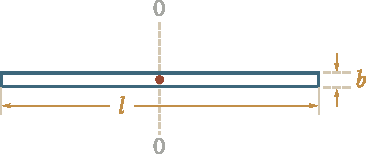
\includegraphics[scale=0.95]{figures/ch_05/fig_5_13.pdf}
			\caption[]{}
			\label{fig:5_13}
		\end{center}
	\end{minipage}
	\hspace{-0.05cm}
	\begin{minipage}[t]{0.5\linewidth}
		\begin{center}
			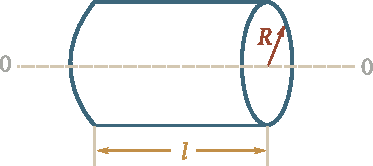
\includegraphics[scale=0.9]{figures/ch_05/fig_5_14.pdf}
			\caption[]{}
			\label{fig:5_14}
		\end{center}
	\end{minipage}
%\vspace{-0.1cm}
\end{figure}

\begin{figure}[t]
	\begin{center}
		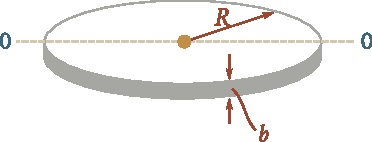
\includegraphics[scale=0.95]{figures/ch_05/fig_5_15.pdf}
		\caption[]{}
		\label{fig:5_15}
	\end{center}
	\vspace{-1.0cm}
\end{figure}

In concluding, we shall give the values of the moments of inertia for selected bodies (the latter are assumed to be homogeneous, $m$ is the mass of the body).
\begin{enumerate}[1.]
	\item The body is a thin long rod with a cross section of any shape. The maximum cross-sectional dimension $b$ of the rod is many times smaller than its length $l$ ($b\sim l$). The moment of inertia relative to an axis perpendicular to the rod and passing through its middle (\fig{5_13}) is
	\begin{equation}\label{eq:5_25}
	I = \frac{1}{12}ml^2.
	\end{equation}

	\item For a disk or cylinder with any ratio of $R$ to $l$ (\fig{5_14}), the moment of inertia relative to an axis coinciding with the geometrical axis of the cylinder is
	\begin{equation}\label{eq:5_26}
	I = \frac{1}{2}mR^2.
	\end{equation}

	\item The body is a thin disk. The thickness of the disk $b$ is many times smaller than the radius of the disk $R$ ($b\sim R$). The moment of inertia relative to an axis coinciding with the diameter of the disk (\fig{5_15}) is
	\begin{equation}\label{eq:5_27}
		I = \frac{1}{4}mR^2.
	\end{equation}

	\item The moment of inertia of a sphere of radius $R$  relative to an axis passing through its centre is
	\begin{equation}\label{eq:5_28}
		I = \frac{2}{5}mR^2.
	\end{equation}
\end{enumerate}

\section{Concept of Inertia Tensor}\label{sec:5_5}

We established in Sec.~\ref{sec:5_3} that for a homogeneous body rotating about an axis of symmetry, the relation between the vectors $\vec{L}$ and $\vec{\omega}$ has a very simple form [\eqn{5_12}]
\begin{equation*}
\vec{L} = I\vec{\omega}
\end{equation*}

\noindent
or
\begin{equation}\label{eq:5_29}
L_x = I\omega_x,\quad L_y = I\omega_y,\quad L_z = I\omega_z.
\end{equation}

\noindent
The explanation is that for such a body the vectors $\vec{L}$ and $\vec{\omega}$ are collinear. In the general case, however, the vectors $\vec{L}$ and $\vec{\omega}$ make an angle differing from zero (see \fig{5_7}), so that the relation between them cannot be expressed by \eqn{5_12}.

Let us try to find a way of relating the vectors $\vec{L}$ and $\vec{\omega}$ analytically in the most general case. We shall proceed from the fact that the magnitudes of $\vec{L}$ and $\vec{\omega}$ are proportional to each other. Indeed, according to \eqn{5_8}, the magnitudes of the elementary vectors $\vec{L}_i$ are proportional to the magnitude of $\vec{\omega}$. Hence, the magnitude of the sum of these vectors is also proportional to $\vec{\omega}$. It is easy to understand that such proportionality is obtained when each component of the vector $\vec{L}$ depends linearly on the components of the vector $\vec{\omega}$:
\begin{align}
L_x &= I_{xx}\omega_x + I_{xy}\omega_y + I_{xz}\omega_z\nonumber\\
L_y &= I_{yx}\omega_x + I_{yy}\omega_y + I_{yz}\omega_z\label{eq:5_30}\\
L_z &= I_{zx}\omega_x + I_{zy}\omega_y + I_{zz}\omega_z.\nonumber
\end{align}

\noindent
Here the quantities $I_{xx}, I_{xy}$, etc. are proportionality constants having the dimension of the moment of inertia [compare with \eqn{5_29}]. When $\vec{\omega}$ increases a certain number of times, each of the components $\omega_x, \omega_y, \omega_z$, and accordingly each of the components $L_x, L_y, L_z$ grows the same number of times, as, consequently, does the vector $\vec{L}$ itself.

The mutual orientation of the vectors $\vec{L}$ and $\vec{\omega}$ is determined by the values of the proportionality constants. Assume, for example, that $I_{xx}=I_{yy}=I_{zz}$, and the remaining constants equal zero. In this case, Eqs.~\eqref{eq:5_30} transform into Eqs.~\eqref{eq:5_29}, \ie, the vectors $\vec{L}$ and $\vec{\omega}$ will be collinear. Now let us assume that the vector $\vec{\omega}$ is directed along the $z$-axis, and the constants $I_{xz}, I_{yz}, I_{zz}$ differ from zero. In this case $\omega_z=\omega, \omega_x=\omega_y=0$. Substitution of these values in Eqs.~\eqref{eq:5_30} yields
\begin{equation*}
L_x = I_{xz}\omega\neq 0,\quad L_y = I_{yz}\omega\neq 0,\quad L_z = I_{zz}\omega\neq 0.
\end{equation*}

\noindent
All three components of the vector $\vec{L}$ differ from zero. Hence, the vector $\vec{L}$ makes a certain angle with the vector $\vec{\omega}$ directed along the $z$-axis.

It follows from the above that in the most general case the relation between the angular momentum and the angular velocity of a body can be expressed with the aid of Eqs.~\eqref{eq:5_30}. Similar equations can be written for any vectors $\vec{a}$ and $\vec{b}$ whose magnitudes are proportional to each other:
\begin{align}
	b_x &= T_{xx} a_x + T_{xy} a_y + T_{xz} a_z\nonumber\\
	b_y &= T_{yx} a_x + T_{yy} a_y + T_{yz} a_z \label{eq:5_31} \\
	b_z &= T_{zx} a_x + T_{zy} a_y + T_{zz} a_z.\nonumber
\end{align}

\noindent
These three equations can be written compactly in the form of a single expression:
\vspace{-12pt}
\begin{equation}\label{eq:5_32}
b_i = \sum_{k=x,y,z} T_{ik} a_k.
\end{equation}

\noindent
Assuming that $i=x$ and performing summation with the subscript $k$ sequentially having the values $x,y,z$, we get the first of the equations~\eqref{eq:5_31}, assuming that $i=y$, we get the second equation, etc.

The combination of the nine quantities $T_{xx}, T_{xy}, \ldots, T_{zz}$ is called a \textbf{tensor of rank two}\footnote{A tensor of rank two is defined as a combination of the nine quantities $T_{xx}, T_{xy}, \ldots, T_{zz}$ that transform according to definite rules upon rotations of the coordinate axes.}, and the operation expressed by Eqs.~\eqref{eq:5_31} is called multiplication of the vector $\vec{a}$ by the tensor $T$. Such multiplication produces a new vector $\vec{b}$.

It is customary practice to write a tensor in the form of a square table\footnote{More commonly known as matrix form --Ed.}:
\begin{equation}\label{eq:5_33}
	T = \begin{pmatrix}
		T_{xx}&T_{xy}&T_{xz}\\
		T_{yx}&T_{yy}&T_{yz}\\
		T_{zx}&T_{zy}&T_{zz}
		\end{pmatrix}
\end{equation}

\noindent
(we can write the subscripts $1, 2, 3$ instead of $x, y, z$). The quantities $T_{xx}, T_{xy}, \ldots$ are defined as the components of the tensor. The components $T_{xx}, T_{yy}, T_{zz}$ along the diagonal of matrix~\eqref{eq:5_33} are called diagonal ones. The values of the components depend on the choice of the coordinate axes onto which the vectors $\vec{a}$ and $\vec{b}$ are projected (the components of these vectors also depend on the choice of the axes).

A comparison of Eqs.~\eqref{eq:5_30} and \eqref{eq:5_31} shows that the constants in Eqs.\eqref{eq:5_30} are the components of a tensor of rank two:
\begin{equation}\label{eq:5_34}
	I = \begin{pmatrix}
		I_{xx}&I_{xy}&I_{xz}\\
		I_{yx}&I_{yy}&I_{yz}\\
		I_{zx}&I_{zy}&I_{zz}
	\end{pmatrix}.
\end{equation}

\noindent
It is called the \textbf{inertia tensor} of a body. This tensor characterizes the inertia properties of a body in rotation.

\begin{figure}[t]
	\begin{center}
		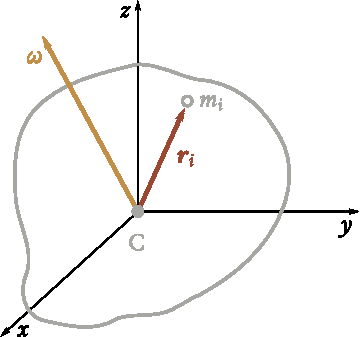
\includegraphics[scale=1.0]{figures/ch_05/fig_5_16.pdf}
		\caption[]{}
		\label{fig:5_16}
	\end{center}
\vspace{-1.0cm}
\end{figure}

To find the values of the components of the inertia tensor, we shall proceed from the definition of the angular momentum of a body:
\begin{equation}\label{eq:5_35}
\vec{L} = \sum_i m_i [\vecprodind{r}{i}{v}{i}]
\end{equation}

\noindent
[see \eqn{5_7}]. We shall plot the vectors $\vec{r}_i$ from the centre of mass of a body (\fig{5_16}). Let us substitute the vector product $\vecprod{\omega}{r}_i$ for the velocity $\vec{v}_i$ in \eqn{5_35} [see \eqn{1_100}]. We get
\begin{equation*}
\vec{L} = \sum_i m_i [\vec{r}_i \times (\vec{\omega} \times \vec{r}_i)].
\end{equation*}

\noindent
We shall now use \eqn{1_35}:
\begin{equation}\label{eq:5_36}
\vec{L} = \sum_i m_i [\vec{\omega}(\vec{r}_i\boldsymbol{\cdot}\vec{r}_i) - \vec{r}_i(\vec{r}_i\boldsymbol{\cdot}\vec{\omega})].
\end{equation}

\noindent
We remind our reader that summation is conducted of all the elementary masses into which we have mentally divided the body.

Let us associate a Cartesian system of coordinates with the body\footnote{It must be stressed that the axes of this system are rigidly associated with the body and rotate together with it.} (see \fig{5_16}) and write the scalar products figuring in \eqn{5_16} through the components of the vectors $\vec{\omega}$ and $\vec{r}_i$ along the axes of this system [see~\eqn{1_23}]. We place the origin of coordinates at the centre of mass of the body C (it must be remembered that we plotted the vectors $\vec{r}_i$ from this point). Taking into account that $r_{xi}=x_i, r_{yi}=y_i, r_{zi}=z_i$, we get
\begin{equation}\label{eq:5_37}
\vec{L} = \sum_i m_i [\vec{\omega}(x_i^2+y_i^2+z_i^2) - \vec{r}_i(x_i\omega_x+y_i\omega_y+z_i\omega_z)].
\end{equation}

\noindent
Let us find the projection of this vector onto the $x$-axis:
\begin{align}
L_x &= \sum_i m_i [\omega_x(x_i^2+y_i^2+z_i^2) - x_i(x_i\omega_x+y_i\omega_y+z_i\omega_z)] \nonumber\\
&= \omega_x\sum_i m_i(y_i^2+z_i^2) - \omega_y\sum_i m_i x_i y_i - \omega_z\sum_i m_i x_i z_i.\label{eq:5_38}
\end{align}

\noindent
In a similar way, we find the projections of the vector $\vec{L}$ onto the axes $y$ and $z$:
\begin{align}
L_y &= -\omega_x\sum_i m_i y_i x_i + \omega_y\sum_i m_i (x_i^2+z_i^2) - \omega_z\sum_i m_i y_i z_i \label{eq:5_39}\\
L_z &= -\omega_x\sum_i m_i z_i x_i - \omega_y\sum_i m_i z_i y_i + \omega_z\sum_i m_i (x_i^2+y_i^2). \label{eq:5_40}
\end{align}

A comparison of the expressions obtained with Eqs.~\eqref{eq:5_30} allows us to find the values of the components of the inertia tensor. Let us write these values at once in the form of a matrix:
\begin{equation}\label{eq:5_41}
	I = \begin{pmatrix}
		\displaystyle\sum_i m_i(y_i^2+z_i^2) & -\displaystyle\sum_i m_i x_i y_i & -\displaystyle\sum_i m_i x_i z_i\\
		-\displaystyle\sum_i m_i y_i x_i & \displaystyle\sum_i m_i (x_i^2+z_i^2) & -\displaystyle\sum_i m_i y_i z_i\\
		-\displaystyle\sum_i m_i z_i x_i & -\displaystyle\sum_i m_i z_i y_i & \displaystyle\sum_i m_i (x_i^2+y_i^2)
	\end{pmatrix}.
\end{equation}

\noindent
The diagonal components of the tensor are the moments of inertia relative to the corresponding coordinate axes considered in the preceding section. These components are called \textbf{axial moments of inertia}. The non-diagonal components are called \textbf{centrifugal moments of inertia}. It must be noted that the non-diagonal components of the tensor~\eqref{eq:5_41} comply with the condition that $I_{xy}=I_{yx}, I_{xz}=I_{zx}, I_{yz}=I_{zy}$. A tensor complying with such a condition is called \textbf{symmetrical}.

In practice, the inertia tensor components are computed with the aid of integration. For example, the component $I_{xx}$ is determined by the formula
\begin{equation*}
	I_{xx} = \int \rho(x,y,z)(y^2+z^2)\,\deriv{V}
\end{equation*}

\noindent
where $\rho(x,y,z)$ is the density, and $\deriv{V}$ is the elementary volume. Integration is performed over the entire volume of the body.

\begin{figure}[t]
	\begin{center}
		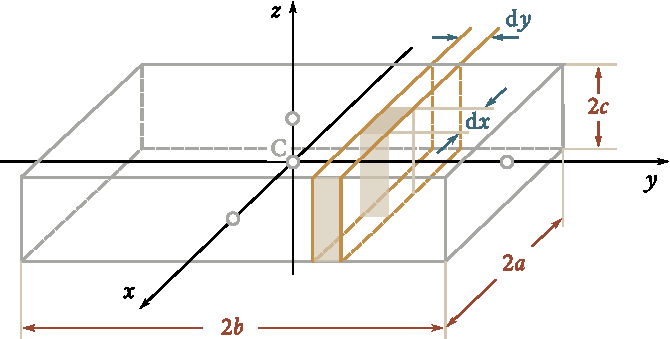
\includegraphics[scale=0.8]{figures/ch_05/fig_5_17.pdf}
		\caption[]{}
		\label{fig:5_17}
	\end{center}
\vspace{-1.0cm}
\end{figure}

Let us find the components of the inertia tensor for a homogeneous rectangular parallelepiped. We select the coordinate axes as shown in \fig{5_17}. The origin of coordinates coincides with the centre of mass of the body C. To calculate the axial moment of inertia $I_{zz}$ we divide our parallelepiped into columns with a base area of $\deriv{x}\,\deriv{y}$. All the elements of such a column have identical values of the coordinates $x$ and $y$. The volume of a column is $2c\,\deriv{x}\,\deriv{y}$, and its mass $\deriv{m}$ is $\rho 2c\,\deriv{x}\,\deriv{y}$. Therefore, the contribution of the column to $I_{zz}$ is determined by the expression
\begin{equation*}
\deriv{I_{zz,\text{column}}} = 2\rho c(x^2+y^2)\deriv{x}\,\deriv{y}.
\end{equation*}

\noindent
Integration of this expression with respect to $x$ gives the contribution to $I_{zz}$ of the layer of length $2a$, width $2c$, and thickness $\deriv{y}$ shown in \fig{5_17}:
\begin{align}
\deriv{I_{zz,\text{layer}}} &= \int_{-a}^{+a} 2\rho c(x^2+y^2)\,\deriv{x}\,\deriv{y}\nonumber\\
&= 2\rho c\,\deriv{y}\int_{-a}^{+a} x^2\,\deriv{x} + 2\rho cy^2\,\deriv{y}\int_{-a}^{+a}\deriv{x} \nonumber\\
&= \left(\frac{4}{3}\rho ca^3 + 4\rho cay^2\right)\,\deriv{y}\label{eq:5_42}
\end{align}

\noindent
(the density $\rho$ does not depend on the coordinates $x$, $y$, and $z$ because the body is homogeneous).

Finally, integrating \eqn{5_42} with respect to $y$, we get $I_{zz}$ for the entire parallelepiped of mass $m$:
\begin{align*}
I_{zz} &= \int_{-b}^{+b} \left(\frac{4}{3}\rho ca^3+4\rho cay^2\right)\,\deriv{y} = \frac{4}{3}\rho ca^3 \int_{-b}^{+b}\deriv{y} + 4\rho ca \int_{-b}^{+b} y^2 \,\deriv{y}\\
&= \frac{8}{3}\rho ca^3b + \frac{8}{3}\rho cab^3 = \frac{1}{3} \rho (2a)(2b)(2c)(a^2+b^2) = \frac{1}{3}m(a^2+b^2).
\end{align*}

\noindent
Similar calculations give $I_{xx}=m(b^2+c^2)/3$, and $I_{yy}=m(a^2+c^2)/3$.

Now let us calculate one of the centrifugal moments, for instance $I_{xy}$. The contribution to this moment of a column with the base $\deriv{x}\,\deriv{y}$ is
\begin{equation*}
\deriv{I_{xy,\text{column}}} = -\rho xy2c\,\deriv{x}\,\deriv{y}
\end{equation*}

\noindent
and the contribution of a layer is
\begin{equation*}
\deriv{I_{xy,\text{layer}}} = -2\rho cy\,\deriv{x} \int_{-a}^{+a}x\,\deriv{y} = 0.
\end{equation*}

\noindent
Accordingly, the moment of the entire parallelepiped equals zero. A similar result is also obtained for the other centrifugal moments. Thus, when we choose the coordinate axes as shown in \fig{5_17}, the inertia tensor of a homogeneous rectangular parallelepiped has the form
\begin{equation}\label{eq:5_43}
	I = \begin{pmatrix}
		I_x&0&0\\
		0&I_y&0\\
		0&0&I_z
	\end{pmatrix}
\end{equation}

\noindent
(we have retained only one of the two identical subscripts for the diagonal components).

\begin{figure}[t]
	\begin{center}
		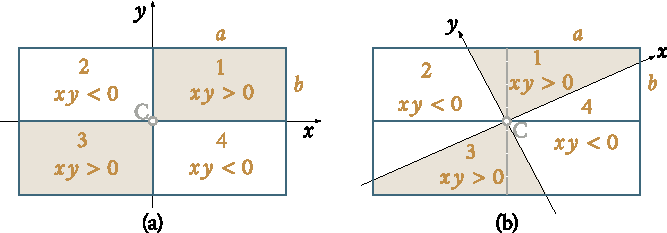
\includegraphics[scale=0.9]{figures/ch_05/fig_5_18.pdf}
		\caption[]{}
		\label{fig:5_18}
	\end{center}
	\vspace{-0.9cm}
\end{figure}

We obtained such a result because we choose the principal axes of inertia (see Sec.~\ref{sec:5_3}) of the parallelepiped as the coordinate axes. Upon a different choice of the coordinate axes, the centrifugal moments of inertia will differ from zero. The following reasoning will convince us that this is true. When we choose the axes as shown in \fig{5_18}a, the areas of rectangles $1, 2, 3$, and $4$ are the same. On two of them, the product $xy$ is positive, and on two negative. As a result, the integral of $xy$ taken over the entire area vanishes. When we choose the axes as shown in \fig{5_18}b, the areas of the shaded figures $1$ and $3$ are less than those of the unshaded figures $2$ and $4$ (because $a>b$). Therefore, the integral of $xy$ taken over the entire area will differ from zero. Accordingly, the centrifugal moment $I_{xy}$ also differs from zero.

The result obtained is common for all bodies regardless of their shape and mass distribution. If we take the principal axes of inertia of a body as the coordinate axes, the inertia tensor has the form given by \eqn{5_43}. The quantities $I_x, I_y, I_z$ [but not $I_{xx}, I_{yy}, I_{zz}$ in \eqn{5_34}; upon rotation of the coordinate axes all the tensor components change, the diagonal ones included] are called the \textbf{principal moments of inertia} of a body. It must be underlined that the axial moments calculated not about arbitrary axes, but about the principal ones, are called the principal moments of inertia.

The principal axes of inertia are mutually perpendicular and intersect at the centre of mass of a body. In the general case (when $I_x\neq I_y\neq I_z$), we can choose these axes in a single way. For a spherical top (\ie, a body for which $I_x=I_y=I_z$, see Sec.~\ref{sec:5_3}), the position of the principal axes is absolutely indeterminate. For a symmetrical top ($I_x=I_y\neq I_z$), only the $z$-axis is fixed, the other
two axes being indeterminate.

Assume that a body rotates about one of its principal axes of inertia, say about the $z$-axis. Selecting the principal axes as the coordinate ones, we have $\omega_z=\omega, \omega_x=\omega_y=0$. Since the inertia tensor has the form of \eqn{5_43} when the coordinate axes are chosen in this way, Eqs.~\eqref{eq:5_30} give the following values of the components of the angular momentum of a body:
\begin{equation*}
L_x = L_y = 0,\quad L_z=I_z\omega.
\end{equation*}

\noindent
Consequently, the vector $\vec{L}$ has the same direction as $\vec{\omega}$. The same result is obtained for rotation of a body about the other principal axes. In all these cases, we arrive at \eqn{5_12}:
\begin{equation*}
\vec{L} = I\vec{\omega}
\end{equation*}

\noindent
where $I$ is the corresponding principal moment of inertia of the body. In Sec.~\ref{sec:5_3}, we obtained \eqn{5_12} for a homogeneous body rotating about its axis of symmetry. Now we have established that this equation holds when an arbitrary body rotates about one of its principal axes of inertia.

In conclusion, let us determine when the equation $\dot{\vec{L}}=\vec{M}$ [see \eqn{3_118}], which is always correct, can be written in the form
\begin{equation}\label{eq:5_44}
I \vec{\alpha} = \vec{M}.
\end{equation}

We may do this first of all when a body rotates about a principal axis, and the moment of the forces $\vec{M}$ is directed along this axis. Indeed, in this case, the moment $\vec{M}$ produces the increment $\deriv{\vec{L}}$ that is collinear with $\vec{L}$ ($\deriv{\vec{L}}=\vec{M}\,\deriv{t}$). Hence, rotation constantly takes place about a principal axis so that the relation $\vec{L}=I\vec{\omega}$ is never violated. In this case, however, \eqn{5_44} gives nothing new in comparison with the formula
\begin{equation}\label{eq:5_45}
	I\alpha_z = M_z.
\end{equation}

\noindent
Here $z$ is the axis of rotation.

When $\vec{M}$ is not collinear with $\vec{L}$ (for example, when $\vec{M}$ is perpendicular to $\vec{L}$, the axis of rotation moves relative to the body with time. Consequently, even provided that the relation $\vec{L}=I\vec{\omega}$ is obeyed at the initial moment, this relation stops being obeyed with time, and \eqn{5_44} loses its meaning. The displacement of the axis of rotation relative to the body is of no significance only when the body is a spherical top. For such a top, any axis is a principal one and has the same value of the moment of inertia $I$. Therefore, \eqn{5_44} holds for any mutual direction of the vectors $\vec{M}$ and $\vec{\omega}$.

\begin{figure}[t]
	\begin{center}
		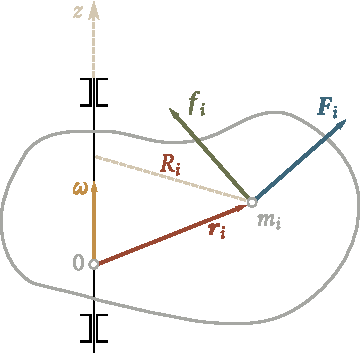
\includegraphics[scale=1]{figures/ch_05/fig_5_19.pdf}
		\caption[]{}
		\label{fig:5_19}
	\end{center}
	\vspace{-0.6cm}
\end{figure}

\section{Kinetic Energy of a Rotating Body}\label{sec:5_6}

Let us begin with a consideration of the rotation of a body about a fixed axis, which we shall call the $z$-axis (\fig{5_19}). The linear velocity of the elementary mass $m_i$ is $v_i=\omega R_i$ where $R_i$ is the distance from the mass $m_i$ to the $z$-axis. Consequently, we get the following expression for the kinetic energy of the $i$-th elementary mass:
\begin{equation*}
	E_{\text{k},i} = \frac{m_i v_i^2}{2} = \frac{1}{2}m_i \omega^2 R_i^2.
\end{equation*}

\noindent
The kinetic energy of a body is composed of the kinetic energies of its parts:
\begin{equation*}
	E_{\text{k}} = \sum_i E_{\text{k},i} = \frac{1}{2}\omega^2 \sum_i m_i R_i^2.
\end{equation*}

\noindent
The sum in the right-hand side of this equation is the moment of inertia of the body $I_z$ relative to the axis of rotation. The kinetic energy of a body rotating about a fixed axis thus equals
\begin{equation}\label{eq:5_46}
	E_{\text{k}} = \frac{1}{2} I_z \omega^2.
\end{equation}

Assume that the mass $m_i$ experiences\footnote{The resultant force $\vec{f}_i+\vec{F}_i$ is in a plane perpendicular to the axis of rotation.} the internal force $\vec{f}_i$, and the external force $\vec{F}_i$ (see \fig{5_19}). According to \eqn{3_16}, these forces do the following work during the time $\deriv{t}$:
\begin{equation*}
\deriv{A_i} = \vecdotind{f}{i}{v}{i}\,\deriv{t} + \vecdotind{F}{i}{v}{i}\,\deriv{t} = \vec{f}_i\boldsymbol{\cdot}(\vecprod{\omega}{r}_i)\,\deriv{t} + \vec{F}_i\boldsymbol{\cdot}(\vecprod{\omega}{r}_i)\,\deriv{t}.
\end{equation*}

\noindent
Performing a cyclic transposition of the multipliers in the scalar triple products [see \eqn{1_34}] we get
\begin{equation}\label{eq:5_47}
\deriv{A_i} = \vec{\omega}\,\boldsymbol{\cdot}(\vecprodind{r}{i}{f}{i})\,\deriv{t} + \vec{\omega}\boldsymbol{\cdot}(\vecprodind{r}{i}{F}{i})\,\deriv{t} = \vecdot{\omega}{M}_{\text{int},i}\,\deriv{t} + \vecdot{\omega}{M}_i\,\deriv{t}
\end{equation}

\noindent
where $\vec{M}_{\text{int},i}$ is the moment of an internal force relative to point $0$, and $\vec{M}_i$ is the similar moment of an external force.

Summation of \eqn{5_47} for all the elementary masses yields the elementary work done on the body during the time $\deriv{t}$:
\begin{equation*}
	\deriv{A} = \sum_i \deriv{A}_i = \vec{\omega}\left(\sum_i \vec{M}_{\text{int},i}\right)\,\deriv{t} + \vec{\omega}\left(\sum_i \vec{M}_{i}\right)\,\deriv{t}.
\end{equation*}

\noindent
The sum of the moments of the internal forces equals zero [see \eqn{3_117}]. Consequently, designating the total moment of the external forces by $\vec{M}$, we get the expression
\begin{equation}\label{eq:5_48}
	\deriv{A} = \vecdot{\omega}{M}\,\deriv{t} = \omega M_z\,\deriv{t}
\end{equation}

\noindent
[we have used \eqn{1_21}, taking into account that $M_{\omega} = M_z$]. Finally, since $\omega\,\deriv{t}$ is the angle $\deriv{\varphi}$ through which the body turns during the time $\deriv{t}$, we have
\begin{equation}\label{eq:5_49}
	\deriv{A} = M_z\,\deriv{\varphi}.
\end{equation}

\noindent
The sign of the work depends on that of $M_z$, \ie, on the sign of the projection of the vector $\vec{M}$ onto the direction of the vector $\vec{\omega}$.

Thus, internal forces do no work when a body rotates, the work of the external forces is determined by \eqn{5_49}. We can arrive at \eqn{5_49} by taking advantage of the fact that the work done by all the forces applied to a body goes to increase its kinetic energy [see \eqn{3_11}]. Differentiating both sides of \eqn{5_46}, we obtain
\begin{equation*}
	\deriv{E_{\text{k}}} = I_z\omega\,\deriv{\omega} = I_z\omega\dot{\omega}\,\deriv{t}.
\end{equation*}

\noindent
According to \eqn{5_15}, $I_z\dot{\omega}=M_z$, and the product $\omega\,\deriv{t}$ equals $\deriv{\varphi}$. Hence, substituting $\deriv{A}$ for $\deriv{E_{\text{k}}}$ we arrive at \eqn{5_49}.

Table~\ref{table:5_1} compares the formulas of mechanics of rotation with similar formulas of mechanics of translation (mechanics of a particle). This comparison shows that in all cases of rotation the part of mass is played by the moment of inertia, the part of force by the moment of a force, the part of momentum by the angular momentum, and so on.

\begin{table}[!b]
	\renewcommand{\arraystretch}{1.2}
	\caption{}
	\vspace{-0.6cm}
	\label{table:5_1}
	\begin{center}\resizebox{0.92\linewidth}{!}{
			\begin{tabular}{ll}
				\toprule[1pt]
				\textbf{Translation} & \textbf{Rotation}\\
				\midrule[0.5pt]\midrule[0.5pt]
				$\vec{v} =\,$ linear velocity & $\vec{\omega} = \,$ angular velocity\\
				$\vec{a}=\dot{\vec{v}} =\,$ linear acceleration & $\vec{\alpha}=\dot{\vec{\omega}} =\,$ angular acceleration\\
				$m=\,$ mass & $I_z=\,$ moment of inertia\\
				$\vec{p}=m\vec{v}=\,$ momentum & $L_z=I_z\omega=\,$ angular momentum\\
				$\vec{F}=\,$ force & $\vec{M}$ or $M_z=\,$ moment of force\\
				$\dot{\vec{p}}=\vec{F}$ & $\dot{\vec{L}}=\vec{M}$\\
				$m\vec{a}=\vec{F}$ & $I\alpha_z=M_z$\\
				$E_{\text{k}}=\frac{1}{2}mv^2$ & $E_{\text{k}}=\frac{1}{2}I\omega^2\,$ (for a fixed axis of rotation)\\
				$\deriv{A}=F_{s}\,\deriv{s}$ & $\deriv{A}=M_z\,\deriv{\varphi}$\\
				\bottomrule[1pt]
			\end{tabular}
			%	\end{center}
	}\end{center}
\end{table}

We obtained \eqn{5_46} for the case when a body rotates about a stationary axis fixed in the body. Now let us assume that a body rotates arbitrarily relative to a fixed point coinciding with its centre of mass. We shall rigidly associate a Cartesian system of coordinates with the body and place its origin at the centre of mass. The velocity of the $i$-th elementary mass is $\vec{v}_i=\vecprod{\omega}{r}_i$. Consequently, we can write the following expression for the kinetic energy of the body:
\begin{equation*}
	E_{\text{k}} = \frac{1}{2}\sum_i m_iv_i^2 = \frac{1}{2}\sum_i m_i (\vecprod{\omega}{r}_i)^2 = \frac{1}{2}\sum_i m_i \omega^2 r_i^2\sin^2\varphi_i
\end{equation*}

\noindent
where $\varphi_i$ is the angle between the vectors $\vec{\omega}$ and $\vec{r}_i$. Substituting $1-\cos^2\varphi_i$ for $\sin^2\varphi_i$, and taking into account that $\omega r_i\cos\varphi=\vecdot{\omega}{r}_i$, we have
\begin{equation*}
	E_{\text{k}} = \frac{1}{2}\sum_i m_i [\vec{\omega}^2\vec{\cdot}\vec{r}_i^2 - (\vecdot{\omega}{r}_i)^2]^2.
\end{equation*}

\noindent
Let us write out the scalar products through the projections of the vectors $\vec{\omega}$ and $\vec{r}_i$ onto the axes of the coordinate system associated with the body:
\begin{align*}
	E_{\text{k}} &= \frac{1}{2}\sum_i m_i \left[(\omega_x^2+\omega_y^2+\omega_z^2)(x_i^2+y_i^2+z_i^2) \right.\\
	&\quad\quad\left. - (\omega_x x_i+\omega_y y_i+\omega_z z_i)(\omega_x x_i+\omega_y y_i+\omega_z z_i)\right]\\
	&= \frac{1}{2}\sum_i m_i \left[(\omega_x^2+\omega_y^2+\omega_z^2)(x_i^2+y_i^2+z_i^2)  \right.\\
	&\quad\quad\left. -\omega_x^2x_i^2 - \omega_x\omega_yx_iy_i - \omega_x\omega_zx_iz_i - \omega_y\omega_xy_ix_i - \omega_y^2y_i^2   \right.\\
	&\quad\quad\quad\left. - \omega_y\omega_zy_iz_i - \omega_z\omega_xz_ix_i - \omega_z\omega_yz_iy_i - \omega_z^2z_i^2\right].
\end{align*}

\noindent
Finally, combining addends with identical products of the angular velocity components and putting these products outside the sums, we get

\begin{align*}
	E_{\text{k}} &= \frac{1}{2}\left[(\omega_x^2 \sum_i m_i (y_i^2+z_i^2) + \omega_y^2 \sum_i m_i (x_i^2+z_i^2) + \omega_z^2 \sum_i m_i (x_i^2+y_i^2) \right.\\
	&\quad\quad\left. - \omega_x\omega_y \sum_i m_ix_iy_i - \omega_x\omega_z \sum_i m_i x_iz_i - \omega_y\omega_x \sum_i m_i y_ix_i \right.\\
	&\quad\quad\quad\left. -\omega_y\omega_z \sum_i m_i y_iz_i - \omega_z\omega_x \sum_i m_i z_ix_i - \omega_z\omega_y \sum_i m_i z_iy_i\right].
\end{align*}

The sums by which the products of the angular velocity components are multiplied are the components of the inertia tensor [see \eqn{5_41}]. Hence, we have arrived at the equation
\begin{align}
	E_{\text{k}} &= \frac{1}{2}\left[I_{xx}\omega_x^2 + I_{xy}\omega_x\omega_y + I_{xz}\omega_x\omega_z + I_{yx}\omega_y\omega_x \right.\nonumber\\
	&\quad\quad\left. + I_{yy}\omega_y^2 + I_{yz}\omega_y\omega_z + I_{zx}\omega_z\omega_x + I_{zy}\omega_z\omega_y + I_{zz}\omega_z^2\right].\label{eq:5_50}
\end{align}

\noindent
This equation can be written in the form
\begin{equation}\label{eq:5_51}
	E_{\text{k}} = \frac{1}{2}\sum_{i,k=x,y,z} I_{ik}\omega_i\omega_k.
\end{equation}

\noindent
In summation, the subscripts $i$ and $k$ are sequentially given the values $x, y, z$ independently of each other.

If the axes of a coordinate system associated with a body are chosen so that they coincide with the principal axes of inertia of the body, the centrifugal moments of inertia will vanish, and \eqn{5_50} will become simplified as follows:
\begin{equation}\label{eq:5_52}
	E_{\text{k}} = \frac{1}{2}(I_x\omega_x^2 + I_y\omega_y^2 + I_z\omega_z^2).
\end{equation}

\noindent
Here $I_x, I_y, I_z$ are the principal moments of inertia of the body. For a spherical top, these moments have the identical value I so that \eqn{5_52} becomes $E_{\text{k}}=I\omega^2/2$ [compare with \eqn{5_46}]. When an arbitrary body rotates about one of the principal axes of inertia, say the $z$-axis, we have $\omega_z=\omega, \omega_x\omega_y=0$, and \eqn{5_52} transforms into~\eqn{5_46}. Thus, the kinetic energy of a rotating body equals half the product of the moment of inertia and the square of the angular velocity in three cases: (1) for a body rotating about a fixed axis, (2) for a body rotating about one of the principal axes of inertia, and (3) for a spherical top. In all other cases, the kinetic energy is determined by more complicated equations~\eqref{eq:5_50} or \eqref{eq:5_52}.

\section{Kinetic Energy of a Body in Plane Motion}\label{sec:5_7}

\vspace{-5pt}

The plane motion of a body can be represented as the superposition of two mo\-tions---translation with a velocity $\vec{v}_0$ and rotation about the relevant axis with the angular velocity $\vec{\omega}$ (see Sec.~\ref{sec:5_1}). By \eqn{5_1}, the velocity of the $i$-th elementary mass of a body is
\begin{equation*}
	\vec{v}_i = \vec{v}_0 + \vecprod{\omega}{r}_i
\end{equation*}

\noindent
where $\vec{v}_0$ is the velocity of a certain point $0$ of the body, and $\vec{r}_i$ is the position vector determining the position of the elementary mass with respect to point $0$.

The kinetic energy of the $i$-th elementary mass is
\begin{equation*}
	E_{\text{k},i} = \frac{1}{2}m_i v_i^2 = \frac{1}{2}m_i (\vec{v}_0 + \vecprod{\omega}{r}_i)^2.
\end{equation*}

\noindent
Squaring the expression in parenthesis, we get
\begin{equation*}
	E_{\text{k},i} = \frac{1}{2}m_i \left[v_0^2 + 2\vec{v}_0\vec{\cdot}(\vecprod{\omega}{r}_i) + (\vecprod{\omega}{r}_i)^2\right].
\end{equation*}

\noindent
The vector product of $\vec{\omega}$ and $\vec{r}_i$ has a magnitude equal to $\omega R_i$, where $R_i$ is the distance to the mass $m_i$ from the axis of rotation [see \fig{1_33} and the text preceding \eqn{1_100}]. Consequently, the third addend in the brackets equals $\omega^2R_i^2$. Let us perform a cyclic transposition of the multipliers in the second addend [see \eqn{1_34}]. As a result, we obtain
\begin{equation}\label{eq:5_53}
	E_{\text{k},i} = \frac{1}{2}m_i \left[v_0^2 + 2(\vec{v}_0\times\vec{\omega})\vec{\cdot}\vec{r}_i + \omega^2 R_i^2\right].
\end{equation}

To obtain the kinetic energy of a body, we find the sum of \eqn{5_53} for all the elementary masses, putting the constant factors outside the sum:
\begin{equation*}
	E_{\text{k}} = \frac{1}{2} v_0^2 \sum_i m_i + (\vec{v}_0\times\vec{\omega})\vec{\cdot}\sum_i m_i\vec{r}_i + \frac{1}{2}\omega^2 \sum_i m_iR_i^2.
\end{equation*}

\noindent
The sum of the elementary masses $\sum_i m_i$ is the mass of the body $m$. The expression $\sum_i m_i\vec{r}_i$ is the product of the mass of the body and the position vector $\vec{r}_{\text{C}}$ of the centre of mass of the body. Finally, $\sum_i m_iR_i^2$ is the moment of inertia of the body $I_0$ relative to an axis passing through point $0$. We can therefore write that
\begin{equation}\label{eq:5_54}
	E_{\text{k}} = \frac{1}{2} mv_0^2 + m\vec{r}_{\text{C}}\vec{\cdot}(\vec{v}_0\times\vec{\omega}) + \frac{1}{2} I_0\omega^2.
\end{equation}

If we take the centre of mass of the body as point $0$, the position vector $\vec{r}_{\text{C}}$ will equal zero, and the second addend will vanish. Consequently, designating by $\vec{v}_{\text{C}}$ the velocity of the centre of mass, and by $I_{\text{C}}$ the moment of inertia of the body relative to an axis passing through point C, we get the following expression for the kinetic energy of the body:
\begin{equation}\label{eq:5_55}
	E_{\text{k}} = \frac{1}{2}m v_{\text{C}}^2 + \frac{1}{2} I_{\text{C}} \omega^2.
\end{equation}

Thus, the kinetic energy of the body in plane motion consists of the energy of translation with a velocity equalling that of the centre of mass and the energy of rotation about an axis passing through the centre of mass of the body.

\section{Application of the Laws of Dynamics of a Body}\label{sec:5_8}

The motion of a rigid body is described by two equations (\eqref{eq:5_6} and \eqref{eq:3_118}) that have already been given in previous sections:
\begin{align*}
	m\vec{a}_{\text{C}} &= \sum\vec{F}_{\text{ext}}\\
	\dot{\vec{L}} &= \sum\vec{M}_{\text{ext}}.
\end{align*}

\noindent
The motion of a body is thus determined by the external forces and the moments of these forces acting on it.

\begin{figure}[t]
	\begin{center}
		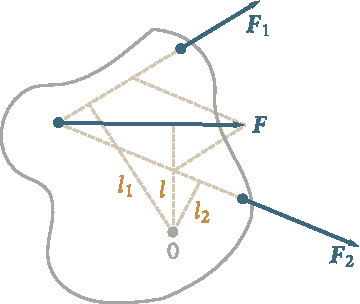
\includegraphics[scale=0.95]{figures/ch_05/fig_5_20.pdf}
		\caption[]{}
		\label{fig:5_20}
	\end{center}
	\vspace{-1.0cm}
\end{figure}

The moments of the forces may be taken relative to any point that is stationary or moving without acceleration. If we took the moment of the external forces relative to a point moving with acceleration, we would in essence write \eqn{3_118} in a non-inertial reference frame. In this case, we must take into consideration the forces of inertia and their moments apart from the external forces due to the interaction of the given body with other bodies.

The points of application of the forces acting on a body may be transferred along the lines of action of the forces because neither the sum of the forces nor their moments will change when this is done (when a force is transferred along the line of its action, the moment arm relative to any point remains unchanged). This permits us to replace several forces with a single one equivalent to them in its action on a body. For example, the two forces $\vec{F}_1$ and $\vec{F}_2$ in one plane (\fig{5_20}) may be replaced with the force $\vec{F}$ equivalent to them. The point of application of the latter may also be chosen arbitrarily on the direction of its action.

A combination of parallel forces acting on a body may be replaced with their resultant equal to the sum of all the forces and applied to a point of the body such that its moment equals the sum of the moments of the separate forces.

Let us find the resultant of the forces of gravity. These forces are applied to all the elements of a body, the force $m_i\vec{g}$ acting on the elementary mass $m_i$. The sum of these forces is $\vec{P}=m\vec{g}$, where $m=\sum_im_i$ is the mass of the body. The total moment of the forces of gravity relative to a certain point $0$ is
\begin{equation*}
	\vec{M} = \sum_i \vec{r}_i \times (m_i \vec{g})
\end{equation*}

\noindent
where $\vec{r}_i$ is the position vector determining the position of the mass $m_i$ with respect to point $0$. Transferring the scalar multiplier $m_i$ from the second member of the product to the first one and then putting the common factor $\vec{g}$ outside the sum, we get
\begin{equation*}
	\vec{M} = \left(\sum_i m_i \vec{r}_i\right) \times \vec{g}.
\end{equation*}

\noindent
The sum in parentheses equals the product of the mass of the body and the position vector $\vec{r}_{\text{C}}$ of the centre of mass C. Hence,
\begin{equation}\label{eq:5_56}
	\vec{M} = (m\vec{r})\times\vec{g} = \vec{r}_{\text{C}} \times (m\vec{g}) = \vec{r}_{\text{C}} \times \vec{P}.
\end{equation}

\noindent
Thus, the total moment of the forces of gravity relative to an arbitrary point $0$ coincides with the moment of the force $m\vec{g}$ applied to point C. Thus, the resultant of the forces of gravity equals $\vec{P}=m\vec{g}$ and is applied to the centre of mass of the body. We must note that this holds only when the field of the forces of gravity is homogeneous within the body [in deriving \eqn{5_56} we considered that $\vec{g}=\text{constant}$].

It follows from \eqn{5_56} that the moment of the forces of gravity relative to the centre of mass equals zero (in this case $\vec{r}_{\text{C}}=0$). The point relative to which the moment of the forces of gravity equals zero is called the \textbf{centre of gravity} of the body. Thus, when the field of gravity forces is homogeneous within a body, the centre of gravity coincides with the centre of mass.

For a homogeneous gravitational field, the forces of gravity applied to different elementary masses have an identical direction and are proportional to $m_i$. The forces of inertia produced in a non-inertial reference frame moving in a straight line relative to inertial frames have the same property. Indeed, in this case, the forces of inertia applied to the elementary masses $m_i$ equal $-m_i\vec{a}_0$, where $\vec{a}_0$ is the acceleration of the non-inertial frame [see \eqn{4_2}]. By repeating the reasoning that led us to \eqn{5_56} (here $-m_i\vec{a}_0$ must be substituted for $m\vec{g}$), we can show that the resultant of the inertia forces equals $-m\vec{a}_0$ and is applied to the centre of mass of the body. It must be stressed that this holds only for reference frames moving in a straight line.

The moment of the inertia forces relative to the centre of mass equals zero (in a frame with translational motion). Therefore, when compiling \eqn{3_118} for the moments taken relative to the centre of mass, the forces of inertia do not have to be taken into consideration.

Let us find the conditions of equilibrium of a rigid body. A body can remain in a state of rest if nothing causes the appearance of translation or rotation. According to Eqs.~\eqref{eq:5_6} and \eqref{eq:3_118}, two conditions are essential and sufficient in this case:
\begin{enumerate}[(1)]
	\item the sum of all the external forces applied to a body must equal zero:
	\begin{equation}\label{eq:5_57}
		\sum\vec{F}_{\text{ext}} = 0.
	\end{equation}

	\item the resultant moment of the external forces relative to any point must equal zero:
	\begin{equation}\label{eq:5_58}
		\sum\vec{M}_{\text{ext}} = 0.
	\end{equation}
\end{enumerate}

When condition~\eqref{eq:5_57} is obeyed, from the equality to zero of the sum of the moments for one point $0$ we get the equality to zero of the sum of the moments relative to any other point $0'$. Indeed, assume that for a certain point $0$ we have
\begin{equation}\label{eq:5_59}
	\sum_i\vec{M}_{i} = \sum_i\vecprodind{r}{i}{F}{i} = 0.
\end{equation}

\noindent
Let us take another point $0'$ whose position relative to $0$ is determined by the vector $\vec{b}$. Examination of \fig{5_21} shows that $\vec{r}_i'=\vec{r}_i-\vec{b}$. Consequently, the sum of the moments relative to point $0'$ is
\begin{equation*}
	\sum_i\vec{M}_{i}' = \sum_i \vec{r}_i'\times\vec{F}_i = \sum_i (\vec{r}_i-\vec{b})\times\vec{F}_i = \sum_i\vecprodind{r}{i}{F}{i} - \sum_i\vec{b}\times\vec{F}_i.
\end{equation*}

\noindent
According to \eqn{5_59}, the first sum equals zero. Factoring out the constant quantity $\vec{b}$ in the second sum, we get the expression $-\left(\vec{b}\times\sum_i\vec{F}_i\right)$ which in view of \eqn{5_57} also vanishes. Thus, from \eqn{5_57} and condition~\eqref{eq:5_59} for point $0$, we get condition~\eqref{eq:5_59} for point $0'$.

\begin{figure}[t]
	\begin{minipage}[t]{0.27\linewidth}
		\begin{center}
			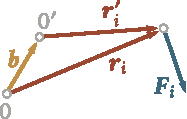
\includegraphics[scale=1]{figures/ch_05/fig_5_21.pdf}
			\caption[]{}
			\label{fig:5_21}
		\end{center}
	\end{minipage}
	\hspace{-0.05cm}
	\begin{minipage}[t]{0.7\linewidth}
		\begin{center}
			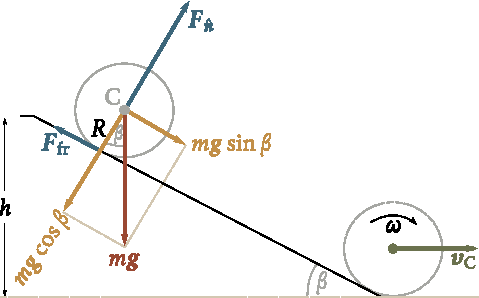
\includegraphics[scale=1]{figures/ch_05/fig_5_22.pdf}
			\caption[]{}
			\label{fig:5_22}
		\end{center}
	\end{minipage}
	\vspace{-0.7cm}
\end{figure}

It must be noted that the vector condition~\eqref{eq:5_58} is equivalent to three scalar ones:
\begin{equation}\label{eq:5_60}
	\sum M_{x,\text{ext}} = 0 ,\quad \sum M_{y,\text{ext}} = 0 ,\quad \sum M_{z,\text{ext}} = 0.
\end{equation}

Thus, the conditions of equilibrium of a rigid body are determined by Eqs.~\eqref{eq:5_57} and~\eqref{eq:5_58}, or by Eqs.~\eqref{eq:5_57} and~\eqref{eq:5_60}.

In conclusion, let us consider an example of the application of the laws of dynamics of a rigid body. Assume that a homogeneous cylinder of radius $R$ and mass $m$ rolls down an inclined plane (\fig{5_22}) without slipping. The angle of inclination of the plane is $\beta$ and its height is $h$ ($h\sim R$). The initial velocity of the cylinder is zero. We are to find the velocity of the centre of mass and the angular velocity of the cylinder at the moment when it reaches the horizontal section. We shall give two variants of the solution.

\textbf{First Variant.} The cylinder will move under the action of three forces---the force $\vec{P}=m\vec{g}$, the force of friction $\vec{F}_{\text{fr}}$, and the force of normal pressure $\vec{F}_{\hatvec{n}}$ (see Sec.~\ref{sec:2_12}. The acceleration of the cylinder in the direction of a normal to the plane is zero. Consequently, the magnitude of the force of normal pressure equals the normal component of the force $\vec{P}$ having the magnitude $mg\cos\beta$.

Friction appears between the cylinder and the plane at the points of their contact. In the absence of slipping, these points of the cylinder are stationary (they form an instantaneous axis of rotation). Hence, the force of friction we are dealing with is a static force of friction. We know from See.~\ref{sec:2_10} that the static force of friction can range from zero to the maximum value $F_0$ that is determined by the product of the coefficient of friction and the force of normal pressure pressing the contacting bodies against each other ($F_0=fmg\cos\beta$). In the case under consideration, the force of friction takes on a value such that slipping will be absent. Slipping will be absent when the cylinder rolls along the plane provided that the linear velocity of the points of contact vanishes. This will occur, in turn, if the velocity of the centre of mass $v_{\text{C}}$ at each moment of time equals the angular velocity of rotation of the cylinder $\vec{\omega}$ multiplied by the radius of the cylinder $R$:
\begin{equation}\label{eq:5_61}
	v_{\text{C}} = \omega R.
\end{equation}

\noindent
The acceleration of the centre of mass $a_{\text{C}}$ will accordingly equal the angular acceleration $\alpha$ multiplied by $R$:
\begin{equation}\label{eq:5_62}
	a_{\text{C}} = \alpha R.
\end{equation}

If the force of friction needed to obey conditions~\eqref{eq:5_61} and~\eqref{eq:5_62} does not exceed the maximum value $F_0$, then the cylinder will roll down the plane without slipping. Otherwise rolling without slipping is impossible.

Equation~\eqref{eq:5_6} in the given case has the form
\begin{equation*}
	m\vec{a}_{\text{C}} = m\vec{g} + \vec{F}_{\text{fr}} + \vec{F}_{\hatvec{n}}.
\end{equation*}

\noindent
Projecting it onto the direction of motion, we get
\begin{equation}\label{eq:5_63}
	ma_{\text{C}} = mg\sin\beta - F_{\text{fr}}.
\end{equation}

For a homogeneous cylinder rotating about an axis of symmetry, $\vec{L}=I\vec{\omega}$. Therefore, \eqn{3_118} can be written in the form
\begin{equation}\label{eq:5_64}
	I\alpha = \sum M_z
\end{equation}

\noindent
where $z$ is the axis of the cylinder [see \eqn{5_51}]. In \eqn{5_64} written relative to the axis of the cylinder, only the moment of the force of friction will differ from zero. The remaining forces including the resultant of the forces of inertia are directed through the axis of the cylinder. As a result, their moments relative to this axis equal zero. Thus, \eqn{5_64} will be written as follows:
\begin{equation}\label{eq:5_65}
	I\alpha = R\,F_{\text{fr}}.
\end{equation}

\noindent
Here $I$ is the moment of inertia of the cylinder relative to its axis equal to $mR^2/2$.

Equations~\eqref{eq:5_63} and~\eqref{eq:5_65} contain three unknown quantities, $F_{\text{fr}}$, $a_{\text{C}}$ and $\alpha$. The last two of them are related by \eqn{5_62} resulting from the absence of friction. By solving the system of equations \eqref{eq:5_62}, \eqref{eq:5_63}, and \eqref{eq:5_65}, we shall find (with account of the fact that $I=mR^2/2$) the values of the required quantities:
\begin{align}
	F_{\text{fr}} &= \frac{1}{3} m g \sin\beta, \label{eq:5_66}\\
	a_{\text{C}} &= \frac{2}{3} g \sin\beta, \label{eq:5_67}\\
	\alpha &= \frac{2}{3}\left(\frac{g}{R}\right)\sin\beta. \label{eq:5_68}
\end{align}

Now that we know the value of the static force of friction needed for rolling down of the cylinder without slipping, we can find the condition at which this rolling is possible. For the cylinder to roll down without slipping, the force~\eqref{eq:5_66} must not exceed the maximum value of the static force of friction $F_0$ equal to $fmg\cos\beta$:
\begin{equation*}
	\frac{1}{3} mg\sin\beta \leqslant mg\cos\beta
\end{equation*}

\noindent
whence
\begin{equation*}
	\tan\beta \leqslant 3f.
\end{equation*}

\noindent
Consequently, if the slope ($\tan\beta$) of the plane exceeds the triple value of the static coefficient of friction between the cylinder and the plane, rolling down cannot occur without slipping.

From the constancy of $a_{\text{C}}$ [see \eqn{5_67}] it follows that the centre of mass of the cylinder moves with uniform acceleration. During the time $t_{\text{r}}$ that it rolls down, the cylinder travels the distance $h/\sin\beta$. In uniformly accelerated motion, the distance, acceleration, and time are related by the equation $s=at^2/2$. Introducing the value of $s$, we get
\begin{equation*}
	\frac{h}{\sin\beta} = \frac{1}{2}a_{\text{C}}t_{\text{r}}^2
\end{equation*}

\noindent
whence, introducing the value of $a_{\text{C}}$ from \eqn{5_67}, we have
\begin{equation*}
	t_{\text{r}} = \frac{1}{\sin\beta}\left(\frac{3h}{g}\right)^{1/2}.
\end{equation*}

\noindent
This time, like $a_{\text{C}}$, does not depend on the mass and radius of the cylinder\footnote{This holds only for a homogeneous solid cylinder.}. It is determined only by the angle of inclination of the plane $\beta$ and the difference between the levels of its edges $h$.

The velocity of the centre of mass when the cylinder reaches the horizontal section will be
\begin{equation*}
	v_{\text{C}} = a_{\text{C}}t_{\text{r}} = \left(\frac{4}{3}gh\right)^{1/2}
\end{equation*}

\noindent
and the angular velocity of the cylinder will be
\begin{equation*}
	\omega = \alpha t_{\text{r}} = \frac{1}{R} \left(\frac{4}{3}gh\right)^{1/2}.
\end{equation*}

We must note that the static force of friction does no work on the cylinder because the points of the cylinder which this force is applied to are stationary at each moment of time [see \eqn{3_16}].

We find for the horizontal plane ($\beta=0$) by Eqs.~\eqref{eq:5_67} and~\eqref{eq:5_68} that the cylinder will travel without acceleration if it is first imparted a certain translational velocity and the corresponding (such that no slipping occurs) angular velocity. The motion will actually be retarded. This is due to the force of rolling friction which is directed so that its moment reduces the angular velocity $\omega$, while the force itself produces a corresponding (again such that no slipping will appear) retardation of the centre of mass. The force of rolling friction does negative work on a rolling body.

In solving the problem on the rolling of a cylinder down an inclined plane, we disregarded rolling friction.

\textbf{Second Variant.} Since the force of friction does no work (we disregard rolling friction), the total energy of the cylinder remains constant. At the initial moment, the kinetic energy is zero, and the potential energy is $mgh$. At the bottom of the inclined plane, the potential energy vanishes but a kinetic energy appears equal to [see \eqn{5_55}]:
\begin{equation*}
	E_{\text{k}} = \frac{mv_{\text{C}}^2}{2} + \frac{I_{\text{C}}\omega^2}{2}.
\end{equation*}

Since slipping is absent, $v_{\text{C}}$ and $\omega$ are related by the expression $v_{\text{C}}=\omega R$. Introducing $\omega=v_{\text{C}}/R$ and $I_{\text{C}}=mR^2/2$ into the expression for the kinetic energy, we get
\begin{equation*}
	E_{\text{k}} = \frac{mv_{\text{C}}^2}{2} + \frac{mv_{\text{C}}^2}{4} = \frac{3}{4}mv_{\text{C}}^2.
\end{equation*}

The total energy at the beginning and end of rolling down the inclined plane must be the same:
\begin{equation*}
	\frac{3}{4}m\,v_{\text{C}}^2 = mgh
\end{equation*}

\noindent
whence
\begin{equation*}
	v_{\text{C}} = \left(\frac{4}{3}gh\right)^{1/2}
\end{equation*}

\noindent
and the angular velocity is
\begin{equation*}
	\omega = \frac{v_{\text{C}}}{R} = \frac{1}{R} \left(\frac{4}{3}gh\right)^{1/2}.
\end{equation*}

Pay attention to how much simpler the second variant of solution is than the first one.

\section{Gyroscopes}\label{sec:5_9}

A gyroscope (or top) is a massive symmetrical body rotating with a great velocity about an axis of symmetry. We shall call this axis the axis of the gyroscope. It is one of the principal axes of inertia. Therefore, if it does not turn in space, the angular momentum is $\vec{L}=I\vec{\omega}$, where $I$ is the moment of inertia relative to the gyroscope axis. Let us now assume that the gyroscope axis rotates with a certain velocity $\vec{\omega}'$. In this case, the resultant rotation of the gyroscope occurs about an axis not coinciding with an axis of symmetry, and the direction of the vector $\vec{L}$ does not coincide with that of the gyroscope axis. If the angular velocity $\omega'$ of the axis is negligibly small in comparison with the angular velocity $\omega$ of the gyroscope itself, however ($\omega'\ll\omega$), then we may assume that the vector $\vec{L}$ is approximately equal to $I\vec{\omega}$ and is directed along the gyroscope axis. In this condition, rotation of the vector $\vec{L}$ and rotation of the gyroscope axis will be equivalent. We shall assume in the following that the condition $\omega'\ll\omega$ is obeyed.

When an attempt is made to turn the gyroscope axis, a distinctive phenomenon is observed called the gyroscopic effect: under the action of forces that ought to cause rotation of the gyroscope axis $00$ about straight line $0'0'$ (\fig{5_23}), the axis turns about straight line $0''0''$ (axis $00$ and straight line $0'0'$ are in the plane of the drawing, and straight line $0''0''$ and the forces $\vec{F}_1$ and $\vec{F}_2$ are at right angles to this plane). The behaviour of the gyroscope, which seems unnatural at first sight, completely conforms with the laws of rotational dynamics. Indeed, the moment of the forces $\vec{F}_1$ and $\vec{F}_2$ is directed along straight line $0'0'$. During the time $\deriv{t}$, the angular momentum of the gyroscope $\vec{L}$ receives the increment $\deriv{\vec{L}}=\vec{M}\,\deriv{t}$, which has the same direction as $\vec{M}$. After the time $\deriv{t}$ elapses, the angular momentum of the gyroscope will equal the resultant $\vec{L}'=\vec{L}+\deriv{\vec{L}}$ in the plane of the figure. The direction of the vector $\vec{L}'$ coincides with the new direction of the gyroscope axis. Thus, the latter will turn about straight line $0''0''$ through a certain angle $\deriv{\varphi}$. It can be seen from \fig{5_23} that $\deriv{\varphi}=|\deriv{\vec{L}}|/L=M\,\deriv{t}/L$. Hence, it follows that the gyroscope axis turned to its new position with the angular velocity $\omega'=\diffin{\varphi}{t}=M/L$. Let us write this relation in the form $M=\omega'L$. The vectors $\vec{M}$, $\vec{L}$ and $\vec{\omega}'$ are mutually perpendicular (the vector $\vec{\omega}'$ is directed along straight line $0''0''$ toward us). The relation between them can therefore be written in the form
\begin{equation}\label{eq:5_69}
	\vec{M} = \vec{\omega}' \times \vec{L}.
\end{equation}

\begin{figure}[t]
	\begin{minipage}[t]{0.55\linewidth}
		\begin{center}
			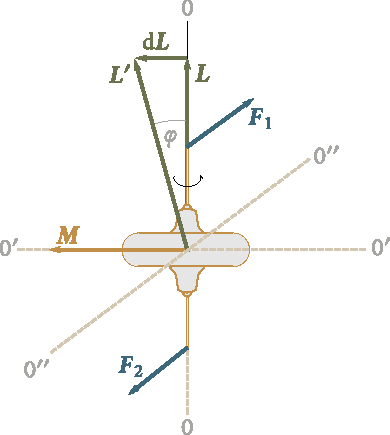
\includegraphics[scale=0.95]{figures/ch_05/fig_5_23.pdf}
			\caption[]{}
			\label{fig:5_23}
		\end{center}
	\end{minipage}
	\hspace{-0.05cm}
	\begin{minipage}[t]{0.45\linewidth}
		\begin{center}
			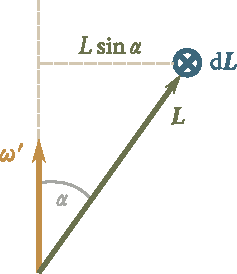
\includegraphics[scale=0.95]{figures/ch_05/fig_5_24.pdf}
			\caption[]{}
			\label{fig:5_24}
		\end{center}
	\end{minipage}
	\vspace{-0.65cm}
\end{figure}

\noindent
We have obtained this equation for the case when the vectors $\vec{\omega}'$ and $\vec{L}$ are mutually perpendicular. It also holds, however, in the most general case. A glance at \fig{5_24} shows that when the gyroscope axis turns about the vector $\vec{\omega}'$ through the angle $\deriv{\varphi}$ the vector $\vec{L}$ receives an increment whose magnitude is $|\deriv{\vec{L}}|=L\sin\alpha\,\deriv{\varphi}$. At the same time $|\deriv{\vec{L}}|=M\,\deriv{t}$. Thus, $L\sin\alpha\,\deriv{\varphi}=M\,\deriv{t}$, whence $M=\omega'L\sin\alpha$. It is easy to see with the aid of \fig{5_24} that in this case \eqn{5_69} holds (the vectors $\vec{\omega}'$ and $\vec{L}$ are in the plane of the figure, the vector $\deriv{\vec{L}}$ is directed beyond the drawing and is therefore depicted by a circle with a cross in it). We remind our reader that \eqn{5_69} is correct only if $\omega'\ll\omega$.

When attempts are made to cause the axis of a gyroscope to turn in a given way, the so-called gyroscopic forces are set up owing to the \textbf{gyroscopic effect}. These forces act on the bearings in which the gyroscope axis rotates. For example, if gyroscope axis $00$ is forcibly turned about straight line $0'0'$ (\fig{5_25}), the gyroscope axis tends to turn about straight line $0''0''$. To prevent this rotation, the forces $\vec{F}_1'$ and $\vec{F}_2'$ acting from the side of the bearings must be applied to the gyroscope axis. According to Newton's third law, the gyroscope axis will act on the bearings with the forces $\vec{F}_1$ and $\vec{F}_2$, and the latter are exactly the gyroscopic forces. Upon forced turning of the gyroscope axis with the angular velocity $\vec{\omega}'$, the moment of the forces with which the bearings act on the axis is determined by \eqn{5_69}. The moment of the gyroscopic forces with which the axis acts on the bearings is
\begin{equation}\label{eq:5_70}
	\vec{M}' = \vec{L}' \times \vec{\omega}.
\end{equation}

\begin{figure}[t]
	\begin{minipage}[t]{0.45\linewidth}
		\begin{center}
			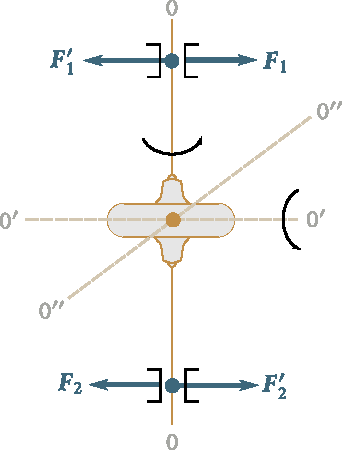
\includegraphics[scale=0.95]{figures/ch_05/fig_5_25.pdf}
			\caption[]{}
			\label{fig:5_25}
		\end{center}
	\end{minipage}
	\hspace{-0.05cm}
	\begin{minipage}[t]{0.55\linewidth}
		\begin{center}
			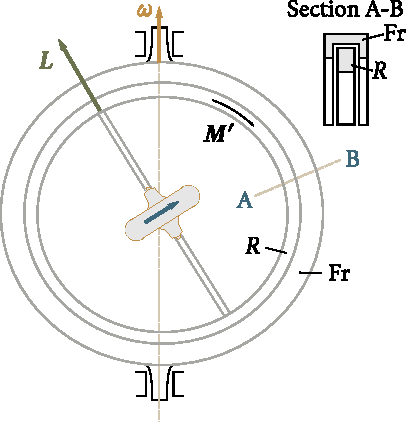
\includegraphics[scale=0.95]{figures/ch_05/fig_5_26.pdf}
			\caption[]{}
			\label{fig:5_26}
		\end{center}
	\end{minipage}
	\vspace{-0.65cm}
\end{figure}

Let us assume that the axis of a gyroscope is fixed in ring $R$ that can freely turn in frame Fr (\fig{5_26}). Let us turn the frame about an axis in its plane with the angular velocity $\vec{\omega}'$. In this case, as we have found out, a moment of gyroscopic forces determined by \eqn{5_70} is produced that acts on the ring. This moment will cause the ring to turn in the frame in the direction indicated by the arrow until the gyroscope axis becomes arranged in the direction of the axis of rotation of the frame and the moment~\eqref{eq:5_70} vanishes. The direction of rotation of the gyroscope itself and the direction in which the frame turns will coincide. When $\vec{L}$ and $\vec{\omega}'$ are directed oppositely, the moment~\eqref{eq:5_70} also vanishes. The corresponding position of the gyroscope axis, however, will be unstable---upon the slightest deviation of the angle between $\vec{L}$ and $\vec{\omega}'$ from \SI{180}{\degree}, the moment $\vec{M}'$ will be set up that will turn the axis until this angle becomes equal to zero.

\begin{figure}[t]
	\begin{center}
		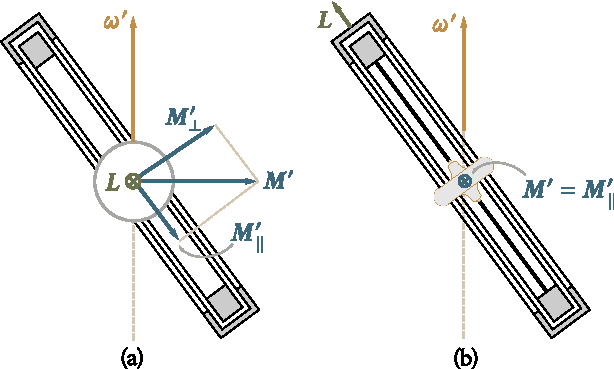
\includegraphics[scale=0.95]{figures/ch_05/fig_5_27.pdf}
		\caption[]{}
		\label{fig:5_27}
	\end{center}
	\vspace{-0.9cm}
\end{figure}

Now let us assume that the frame turns with the angular velocity $\vec{\omega}'$ about an axis not in its plane (\fig{5_27}). In the position of the ring at which the angular momentum of the gyroscope $\vec{L}$ is perpendicular to $\vec{\omega}'$ (\fig{5_27}a), the vector $\vec{M}'$ has the direction shown in the figure. The component $\vec{M}_{\perp}'$ of this vector causes the ring to turn in the frame, and as a result the angle between the vectors $\vec{L}$ and $\vec{\omega}'$ will diminish. The component $\vec{M}_{\parallel}'$ tends to misalign the ring relative to the frame. When the ring occupies a position such that the angle between the vectors $\vec{L}$ and $\vec{\omega}'$ takes on the smallest possible value (\fig{5_27}b), the component $\vec{M}_{\perp}'$ will vanish because in this case the moment of the gyroscopic forces $\vec{M}'$ is in the plane of the ring; this moment cannot produce rotation of the ring in the frame. Thus, under the action of gyroscopic forces, the ring occupies such a position in the frame in which the angle between the gyroscope axis and the axis of rotation of the frame is minimum.

\begin{figure}[t]
	\begin{minipage}[t]{0.4\linewidth}
		\begin{center}
			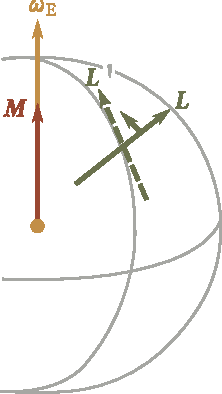
\includegraphics[scale=0.9]{figures/ch_05/fig_5_28.pdf}
			\caption[]{}
			\label{fig:5_28}
		\end{center}
	\end{minipage}
	\hspace{-0.05cm}
	\begin{minipage}[t]{0.6\linewidth}
		\begin{center}
			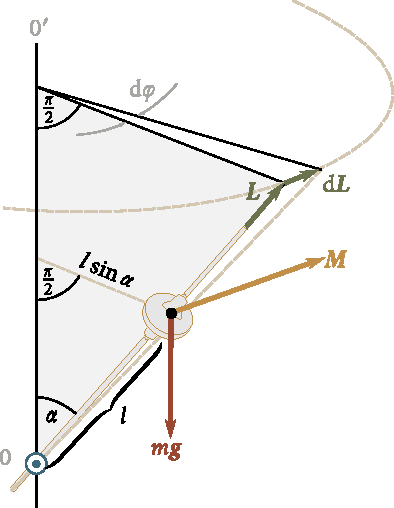
\includegraphics[scale=0.95]{figures/ch_05/fig_5_29.pdf}
			\caption[]{}
			\label{fig:5_29}
		\end{center}
	\end{minipage}
	\vspace{-0.7cm}
\end{figure}

An instrument called the gyrocompass (gyroscopic compass) is based on the behaviour of a gyroscope described above. This instrument is a gyroscope whose axis can freely turn in a horizontal plane. The Earth's daily rotation causes the axis of the gyrocompass to arrange itself in a position such that the angle between this axis and the Earth's axis of rotation will be minimum (\fig{5_28}). In this position, the axis of the gyrocompass will be in a meridian plane and, consequently, line up in a north-south direction. A gyrocompass advantageously differs from its magnetic pointer counterpart in that no corrections have to be introduced into its readings for the so-called magnetic declination (the angle between the magnetic and the geographic meridians). Another advantage is that no measures have to be taken to compensate for the action on the pointer of ferromagnetic objects near the compass (for example, the steel hull of a ship).

Assume that the axis of a gyroscope can freely turn about point $0$ (\fig{5_29}). Let us consider the behaviour of such a gyroscope in the field of forces of gravity. The magnitude of the moment of the forces applied to the gyroscope is
\begin{equation}\label{eq:5_71}
	M = mgl\sin\alpha
\end{equation}

\noindent
where $m$ is the mass of the gyroscope, $l$ is the distance from point $0$ to the centre of mass of the gyroscope and $\alpha$ is the angle made by the gyroscope axis with a vertical line.

The vector $\vec{M}$ is perpendicular to the vertical plane passing through the gyroscope axis (this plane is shaded in \fig{5_29}).

Under the action of the moment $\vec{M}$, the angular momentum $\vec{L}$ changes during the time $\deriv{t}$ by the increment $\deriv{\vec{L}}=\vec{M}\,\deriv{t}$ perpendicular to the vector $\vec{L}$. The amount by which the vector $\vec{L}$ changes upon receiving the increment $\deriv{\vec{L}}$ corresponds to turning of the gyroscope axis such that the angle a does not change. The vertical plane passing through the gyroscope axis turns through the angle $\deriv{\varphi}$.

The vector $\vec{M}$ turns through the same angle in a horizontal plane. As a result, when the time $\deriv{t}$ elapses, the vectors $\vec{L}$ and $\vec{M}$ will have the same mutual arrangement as at the initial moment.

During the next moment $\deriv{t}$, the vector $\vec{L}$ again receives the increment $\deriv{\vec{L}}$ that is perpendicular to the new direction of the vector $\vec{L}$ setting in after the preceding elementary turn, etc. As a result, the gyroscope axis will rotate about the vertical axis passing through point $0$ with the angular velocity $\omega'$. It will describe a cone with an apex angle of $2\alpha$ (compare with \fig{5_24}). (When $\alpha=\pi/2$, the cone degenerates into a plane.) The vector $\vec{L}$ will change only in direction. Its magnitude will be constant because the elementary increments $\deriv{\vec{L}}$ will always be perpendicular to the vector $\vec{L}$\footnote{We can find similar behaviour in the velocity vector when a point moves uniformly along a circle. The vector $\vec{v}$ receives the increment $\deriv{\vec{v}}=\vec{a}_{\hatvec{n}}\,\deriv{t}$ ($\vec{a}_{\hatvec{n}}=\text{constant}$) during the time $\deriv{t}$. As a result, the direction of the vector $\vec{v}$ changes, while its magnitude remains constant.}.

Thus, in the field of forces of gravity, the axis of a gyroscope with a fixed point rotates about a vertical line, describing a cone. Such motion of a gyroscope is called precession. We can find the angular velocity $\omega'$ of precession if we take into account that by \eqn{5_69} $M=\omega'L\sin\alpha$. Equating this value to \eqn{5_71}, we get $\omega'L\sin\alpha=mgl\sin\alpha$, whence
\begin{equation}\label{eq:5_72}
	\omega' = \frac{mgl}{L} = \frac{mgl}{I\omega}.
\end{equation}

\noindent
It follows from \eqn{5_72} that the velocity of precession does not depend on the angle of inclination of the gyroscope axis with respect to a vertical line (on the angle $\alpha$).

We have considered the approximate theory of the gyroscope. According to the strict theory, rotation of the axis about a vertical line is accompanied by oscillations of the axis in a vertical plane. The latter are attended by changes in the angle $\alpha$ ranging from $\alpha_1$ to $\alpha_2$. This wobbling of the axis is called \textbf{nutation}. Depending on the initial conditions, the end of a gyroscope axis draws one of the curves depicted in \fig{5_30} on an imaginary spherical surface. If, for example, after positioning the axis at the angle $\alpha_1$, we make the gyroscope rotate and then release the axis gently, the latter will first lower while rotating about the vertical line. After reaching the angle $\alpha_2$, the axis will begin to rise, and so on (this case is shown in \fig{5_30}b).

\begin{figure}[t]
	\begin{minipage}[t]{0.6\linewidth}
		\begin{center}
			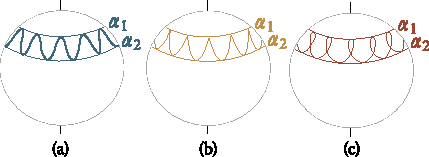
\includegraphics[scale=1]{figures/ch_05/fig_5_30.pdf}
			\caption[]{}
			\label{fig:5_30}
		\end{center}
	\end{minipage}
	\hspace{-0.05cm}
	\begin{minipage}[t]{0.36\linewidth}
		\begin{center}
			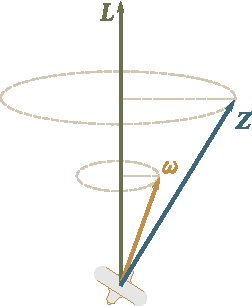
\includegraphics[scale=0.95]{figures/ch_05/fig_5_31.pdf}
			\caption[]{}
			\label{fig:5_31}
		\end{center}
	\end{minipage}
	\vspace{-0.4cm}
\end{figure}


By imparting an initial impetus of a quite definite magnitude and direction to a gyroscope, we can achieve precession of its axis without nutation. Such precession is defined as \textbf{regular}. The amplitude of nutation diminishes with an increasing gyroscope velocity of rotation. Nutation is also absorbed by friction in the support. This is why nutation is often unnoticeable in practice. Precession that is only approximately regular is called \textbf{pseudoregular}.

If point $0$ is at the centre of mass of a gyroscope (see \fig{5_29}), the moment of the force of gravity becomes equal to zero, and we get the so-called free symmetrical top. Owing to the law of conservation, the angular momentum of such a top will change neither in magnitude nor in direction. If we rotate the top about its axis of symmetry, the vectors $\vec{L}$ and $\vec{\omega}$ will have the same direction which remains constant for an infinitely long time. If, however, the top is rotated about an axis not coinciding with any of its principal axes of inertia, the vectors $\vec{L}$ and $\vec{\omega}$ will not coincide (\fig{5_31}). The relevant calculations give us the following results. The vector $\vec{\omega}$ remains constant in magnitude and precesses about the direction of the vector $\vec{L}$ describing a cone. At the same time, the axis of symmetry $z$ of the top precesses, the vectors $\vec{L}$ and $\vec{\omega}$ and the $z$-axis constantly being in one plane. The top rotates about the $z$-axis with the angular velocity $\omega_z=L_z/I_z$, where $L_z$ is the projection of the vector $\vec{L}$ onto the $z$-axis, and $I_z$ is the moment of inertia of the top relative to this axis. The angular velocity of precession is $\omega_{\text{pr}}=L/I$, where $I$ is the identical value of the moments of inertia $I_x$ and $I_y$.
